\documentclass{article}\usepackage[]{graphicx}\usepackage[]{xcolor}
% maxwidth is the original width if it is less than linewidth
% otherwise use linewidth (to make sure the graphics do not exceed the margin)
\makeatletter
\def\maxwidth{ %
  \ifdim\Gin@nat@width>\linewidth
    \linewidth
  \else
    \Gin@nat@width
  \fi
}
\makeatother

\definecolor{fgcolor}{rgb}{0.345, 0.345, 0.345}
\newcommand{\hlnum}[1]{\textcolor[rgb]{0.686,0.059,0.569}{#1}}%
\newcommand{\hlsng}[1]{\textcolor[rgb]{0.192,0.494,0.8}{#1}}%
\newcommand{\hlcom}[1]{\textcolor[rgb]{0.678,0.584,0.686}{\textit{#1}}}%
\newcommand{\hlopt}[1]{\textcolor[rgb]{0,0,0}{#1}}%
\newcommand{\hldef}[1]{\textcolor[rgb]{0.345,0.345,0.345}{#1}}%
\newcommand{\hlkwa}[1]{\textcolor[rgb]{0.161,0.373,0.58}{\textbf{#1}}}%
\newcommand{\hlkwb}[1]{\textcolor[rgb]{0.69,0.353,0.396}{#1}}%
\newcommand{\hlkwc}[1]{\textcolor[rgb]{0.333,0.667,0.333}{#1}}%
\newcommand{\hlkwd}[1]{\textcolor[rgb]{0.737,0.353,0.396}{\textbf{#1}}}%
\let\hlipl\hlkwb

\usepackage{framed}
\makeatletter
\newenvironment{kframe}{%
 \def\at@end@of@kframe{}%
 \ifinner\ifhmode%
  \def\at@end@of@kframe{\end{minipage}}%
  \begin{minipage}{\columnwidth}%
 \fi\fi%
 \def\FrameCommand##1{\hskip\@totalleftmargin \hskip-\fboxsep
 \colorbox{shadecolor}{##1}\hskip-\fboxsep
     % There is no \\@totalrightmargin, so:
     \hskip-\linewidth \hskip-\@totalleftmargin \hskip\columnwidth}%
 \MakeFramed {\advance\hsize-\width
   \@totalleftmargin\z@ \linewidth\hsize
   \@setminipage}}%
 {\par\unskip\endMakeFramed%
 \at@end@of@kframe}
\makeatother

\definecolor{shadecolor}{rgb}{.97, .97, .97}
\definecolor{messagecolor}{rgb}{0, 0, 0}
\definecolor{warningcolor}{rgb}{1, 0, 1}
\definecolor{errorcolor}{rgb}{1, 0, 0}
\newenvironment{knitrout}{}{} % an empty environment to be redefined in TeX

\usepackage{alltt}
\usepackage{hyperref}
\usepackage[margin=0.8in]{geometry}
\usepackage{booktabs}
\usepackage{amsmath}
\usepackage{gensymb}
\usepackage{natbib}
\IfFileExists{upquote.sty}{\usepackage{upquote}}{}
\begin{document}
% \SweaveOpts{concordance=TRUE}

\title{Coringtreespotters ms outline}
\author{Christophe Rouleau-Desrochers}
\date{\today}
\maketitle

% Set CoringTreespotters species shortcut
\newcommand{\Arub}{\textit{A. rubrum}}
\newcommand{\Asac}{\textit{A. saccharum}}
\newcommand{\Afla}{\textit{A. flava}}
\newcommand{\Ball}{\textit{B. alleghaniensis}}
\newcommand{\Bnig}{\textit{B. nigra}}
\newcommand{\Cgla}{\textit{C. glabra}}
\newcommand{\Cova}{\textit{C. ovata}}
\newcommand{\Pdel}{\textit{P. deltoides}}
\newcommand{\Qalb}{\textit{Q. alba}}
\newcommand{\Qrub}{\textit{Q. rubra}}
\newcommand{\Tame}{\textit{T. americana}}   




% <><><><><><><><><><><><><><><><><><><><><><><><><><><><><><><><><><><><><><><>
\section*{Introduction}
% <><><><><><><><><><><><><><><><><><><><><><><><><><><><><><><><><><><><><><><>
\begin{enumerate}
% Paragraph
\item Climate change shift plant phenology
  \begin{enumerate}
  
  \item Earlier spring and delayed autumn lengthens the growing season
  
  \item With longer seasons, trees should grow more
  
  \item Temperate forests offset a large portion of human CO2 emissions
  
  \item Most of that carbon is stored in mature, canopy trees so they are important
  \end{enumerate}

% Paragraph
\item Increased growth with longer seasons may not happen
  \begin{enumerate}
  \item Some new evidence shows trees don't grow more with longer seasons
  
  \item This could mislead carbon models
  
  \item Highlights the need to understand why trees might not grow more
  
  \end{enumerate}
  
% Paragraph
\item Growth strategies (i.e. acquisitive vs conservative) and wood anatomy may guide species responses to GS
  \begin{enumerate}
  
  \item Diffuse vs ring porous species start growth at different time---experience different temperature throughout the season
  
  \item Longer seasons may benefit slow growth species $>$ fast growth species: slow growth rate under good conditions for a long time = increased growth 
  
  \item Different carbon allocation strategies may mute short term growth responses: storage investment vs opportunistic growth
  
  \item Increased C storage in current year, but stored instead of invested in growth: importance of considering multiple years
  
  \end{enumerate}
  
% Paragraph 
\item Previous year conditions can affect the following year's growth
  \begin{enumerate}
  \item Deciduous trees use stored carbon at the beginning of the season
  
  \item Mature trees especially are known to rely on stored carbon for early growth 
  
  \item Thus, effect of environmental conditions on yearly growth can be blurred by a multi-year lag effect %emwJun29 -- nice!
  
  \end{enumerate}
  
% Paragraph
\item Look at growth and GSL relationship in an urban arboretum where drought and competition are limited
  \begin{enumerate}
  \item Will look at 11 species of mature trees across nine years. 
  
  \item GS number of days vs temperature conditions
  
  \item Growth with tree rings and SOS and EOS with leaf phenology from citizen scientists 
  
  \end{enumerate}
\end{enumerate}

% <><><><><><><><><><><><><><><><><><><><><><><><><><><><><><><><><><><><><><><>
% METHODS 
% <><><><><><><><><><><><><><><><><><><><><><><><><><><><><><><><><><><><><><><>
\section*{Methods}
We did a bunch of stuff that I am not outlining. Phenophases by \citep{denny_standardized_2014}

% <><><><><><><><><><><><><><><><><><><><><><><><><><><><><><><><><><><><><><><>
% RESULTS
% <><><><><><><><><><><><><><><><><><><><><><><><><><><><><><><><><><><><><><><>
\clearpage
\section*{Results}

\begin{enumerate}
\item Summary basic information
  \begin{enumerate}

  \item Dataset includes 11 deciduous tree species with leaf phenology data spanning nine years (2016 to 2024) for a total of 
  321 leafout and 
  284 leaf coloring
   observations, yielding 
  278 complete growing seasons (GS) for 
  49 individuals. 
  
  \item Mean summer temperatures spanned 
  21.53$^\circ$C 
  (2017) to 
  23.07$^\circ$C 
  (2020), with an average of
  22.51$^\circ$C across the nine years.

  \item 2020 and 2022 had moderate droughts in the summer (June, July and August) ramped up to severe in September. A moderate drought in June 2016, ramped up to severe in July, then extreme in August and September. 
  
  %emw25Jun -- somewhere in the methods you should say how you checked these early seasons -- or maybe 77 is not really an outlier? Small issue we can fix with a git issue if you need help. 
  \item GSL ranged from 
  77 days ({\Afla} in 
  2018) to 
  194 days ({\Asac} in 
  2021)

  \item GS thermal sum ranged from 
  1048.8 GDD ({\Afla} in 
  2020) to 
  2634.7 GDD ({\Tame} in 
  2016)
  
  \item The earliest leafout day of year was 
  08-Apr ({\Afla} in 
  2021) and the latest, 
  15-May ({\Cova} in 
  2020). The earliest leaf coloring day of year was
  15-Jul ({\Afla} in 
  2021---same individual with earliest leafout) and the latest, 
  06-Nov ({\Tame} in
  2016) 
  
  \item Annual ring widths across years varied from 
  0.43 mm ({\Asac} in 2019) to 
  11.75 mm ({\Tame} in 2019) (Figure \ref{fig:tsboxplot}).
 
\end{enumerate}
% Question 1 --- --- --- --- --- --- --- --- --- --- --- --- --- --- --- --- ---
\item Does tree growth increase with longer growing seasons?
  \begin{enumerate}

  \item No clear trend of growing season length effect across our eleven species and season predictors. %emw25Jun -- 'effect' is stats, not biology, fix this when you make it full text
  %emw25Jun -- all my comments on units (and $z$-score etc.) on wildcrokie apply here also -- I understand RW is easier for you, but I think mm/GSL or such may be easier for your audience; if you feel strongly though and or see this approach in lots of papers, let me know and I will let it go. 
  \item Results reported as means and 90\% uncertainty intervals (UI) that correspond to ring width change in mm on the log scale---henseforth "RW" per scaled predictor (one week (seven days) of average spring growing degree days (GDD); (58.32) for the thermal season, one week of growing season length (GSL) for the calendar season, one week of leafout for the start of season (SOS) and one week of of budset for the end of season (EOS). % crd24June: copied from wildchrokie. Will change according to your edits/suggestions on units throughout.

  \item Longer thermal season did not increase growth for any species and decreased growth for {\Ball} (
  -0.08, UI:
  -0.12,
  -0.03 RW change per scaled GDD; Figure \ref{fig:tsmuplotbspp}a and e; Table \ref{tab:ts_slope_table}).
  
  \item No species responded to longer calendar season (Figure \ref{fig:tsmuplotbspp}b and f; Table \ref{tab:ts_slope_table}).

  \item On a scaled axis (z-scored), both GDD and GSL were similarly predictive (Figure \ref{fig:bsppZscored})

  \end{enumerate}

% Question 2 --- --- --- --- --- --- --- --- --- --- --- --- --- --- --- --- ---
\item Does a warmer thermal season increase growth in the following year?
  \begin{enumerate}
  
  \item Previous year GDD increased growth for {\Ball} (
  0.15, UI:
  0.02,
  0.28 RW change per scaled GDD),
  and decreased growth for {\Bnig} (
  -0.08, UI:
  -0.17,
  0 RW change per scaled GDD; Figure \ref{fig:tsPrvsYr}b)
  
  \item Interestingly, {\Bnig} did not solely respond to current year's conditions (Figure \ref{fig:tsmuplotbspp}a and e; Table \ref{tab:ts_slope_table}), but grew more with warmer thermal season when the previous conditions were considered (
  0.12, UI:
  0.03,
  0.21 RW change per scaled GDD; Figure \ref{fig:tsPrvsYr}a).
  
  \end{enumerate}
  
% Question 3 --- --- --- --- --- --- --- --- --- --- --- --- --- --- --- --- ---
\item Did an earlier start and later end of season increase growth? 

  \begin{enumerate}
  \item An earlier start of season did not increase growth for any species and decreased growth for {\Tame} (
  0.15, UI:
  0.02,
  0.27 RW change per seven SOS days; Figure \ref{fig:tsmuplotbspp}c and g; Table \ref{tab:ts_slope_table}), which did not respond to the thermal or the calendar season.

\item A later end of season did not increase growth for any species and decreased growth for {\Ball} (
-0.09, UI:
-0.16,
-0.01 RW change per seven EOS days; Figure \ref{fig:tsmuplotbspp}d and h; Table \ref{tab:ts_slope_table}), which also decreased growth with warmer thermal season.

\item The estimates were unchanged when using the full or restricted datasets (SOS $n =$
321 and EOS $n =$
284 vs $n=$
278; Figure \ref{fig:tsSOSEOScomparison}b), or when using budburst instead of leafout as the start of the growing season (Figure \ref{fig:buburstVSleafoutTS}c).


\item A later SOS delayed EOS only for {\Pdel} 
(1.04, UI:
0.39,
1.7 EOS change in days per SOS day; Figure \ref{fig:SOSonEOS}
\end{enumerate}

% Question 4 --- --- --- --- --- --- --- --- --- --- --- --- --- --- --- --- ---
\item How did tree growth change across years and tree ids?
  \begin{enumerate}
  
  \item We did not find any clear effect of year on growth (Figure \ref{fig:tsmuplotayear}) and no clear differences of growth across species (Figure \ref{fig:tsxyGDDyr} and Figure \ref{fig:tsxyGSLyr})
  
  \item Growth was similar across individual trees (Figure \ref{fig:tsmuplotatreeid}).

  \end{enumerate}
\end{enumerate}

% Figure mu across all species and climate predictors
\begin{figure}[!ht]
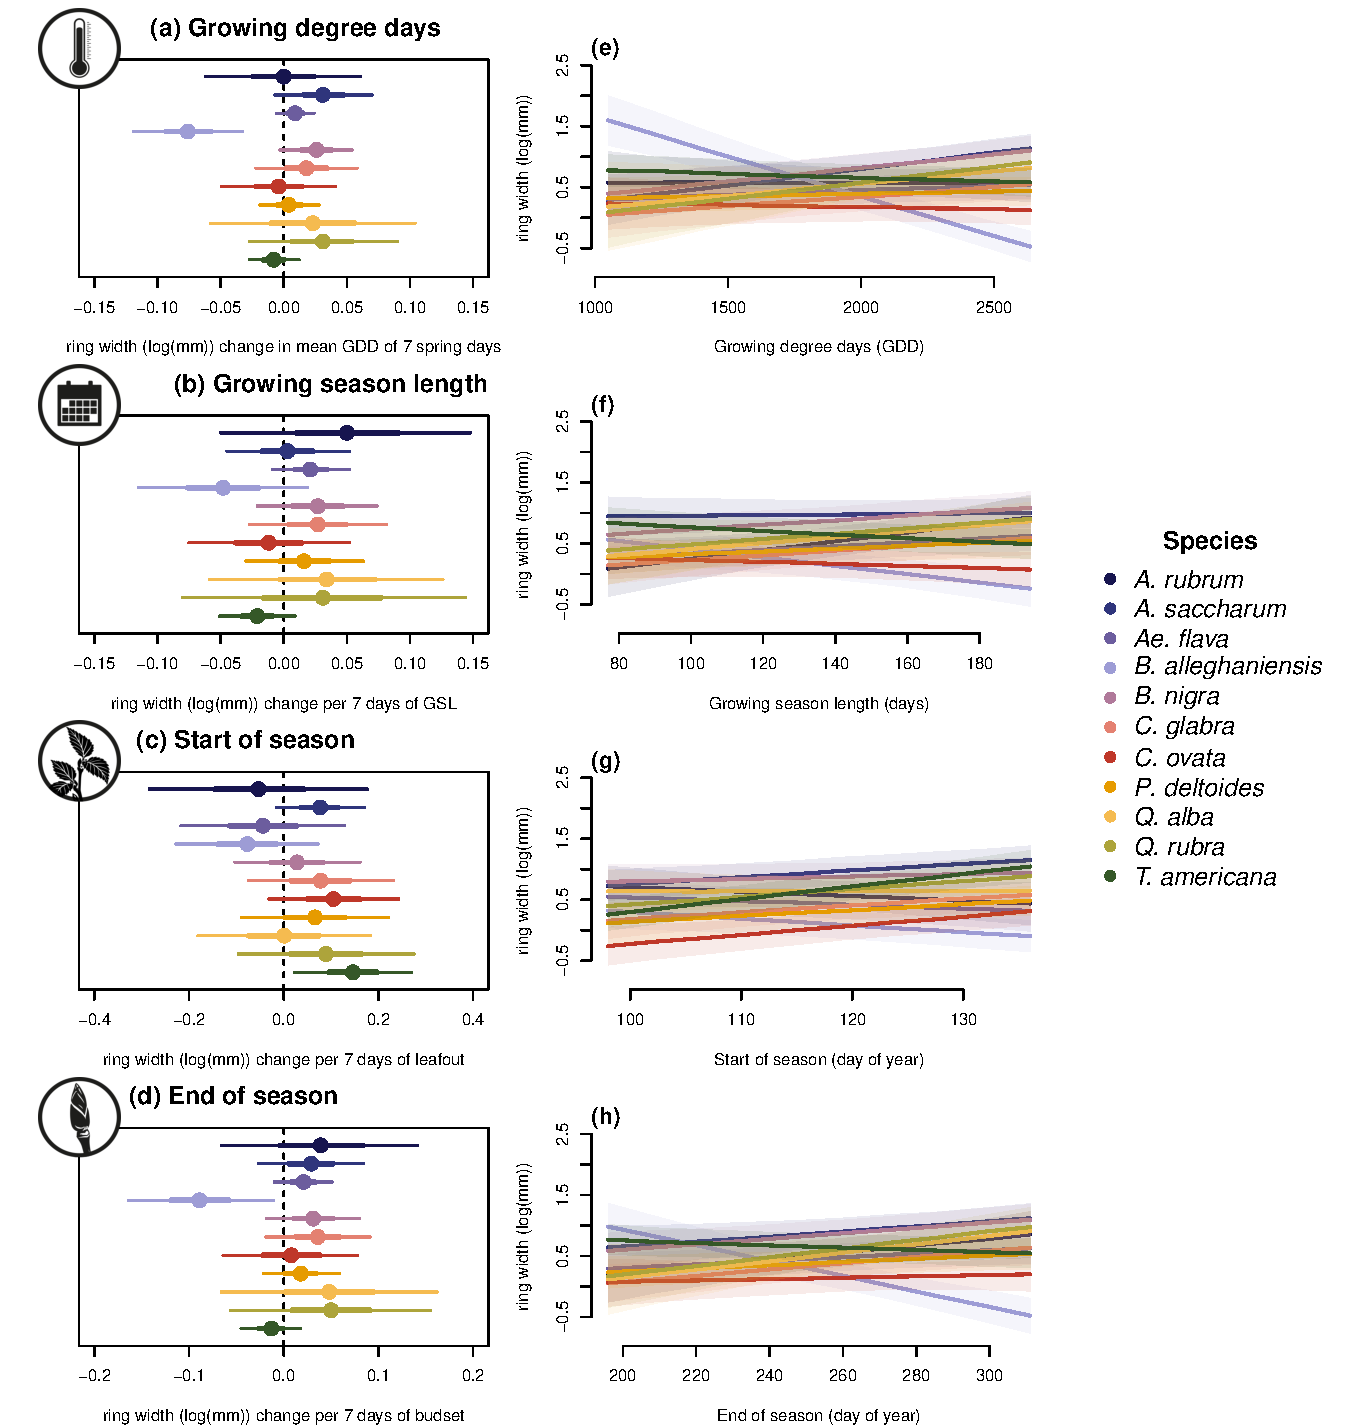
\includegraphics[width=0.8\textwidth]{../../analyses/figures/growthModelsMain/TSmuALLbsppWlines.pdf}
\caption{Estimates of ring width change as a function of four different predictors (growing degree days, GDD (mean daily temperature above 5\degree C); growing season length, GSL; start of season, SOS; end of season, EOS) across our eleven species. The species colors are the same throughout the figures. Panels (a) to (d) represent the model slope estimates for each species, for each predictor, which we represent through ring width change on the log scale per seven average spring days GDD (58.32 GDD; panel a), seven days of GSL (panel b), seven days of leafout (SOS; panel c) and seven days of leaf colouring (EOS; panel d). The dots represent the mean of each species and the lines, the 50\% and 90\% uncertainty intervals (UI; see Table \ref{tab:ts_slope_table} for parameter estimates). Panels (e) to (h) represent the simulated response curves of ring width as a function of each predictor, with the lines depicting the mean response at each simulated predictor value, and the shaded area, the interquantile ranges (25\% and 75\% UI). These model do not include a slope on the previous year GDD (see Figure \ref{fig:tsPrvsYr} for these estimates).}
\label{fig:tsmuplotbspp}
\end{figure}

% Figure mu previous year and current year
\begin{figure}[!ht]
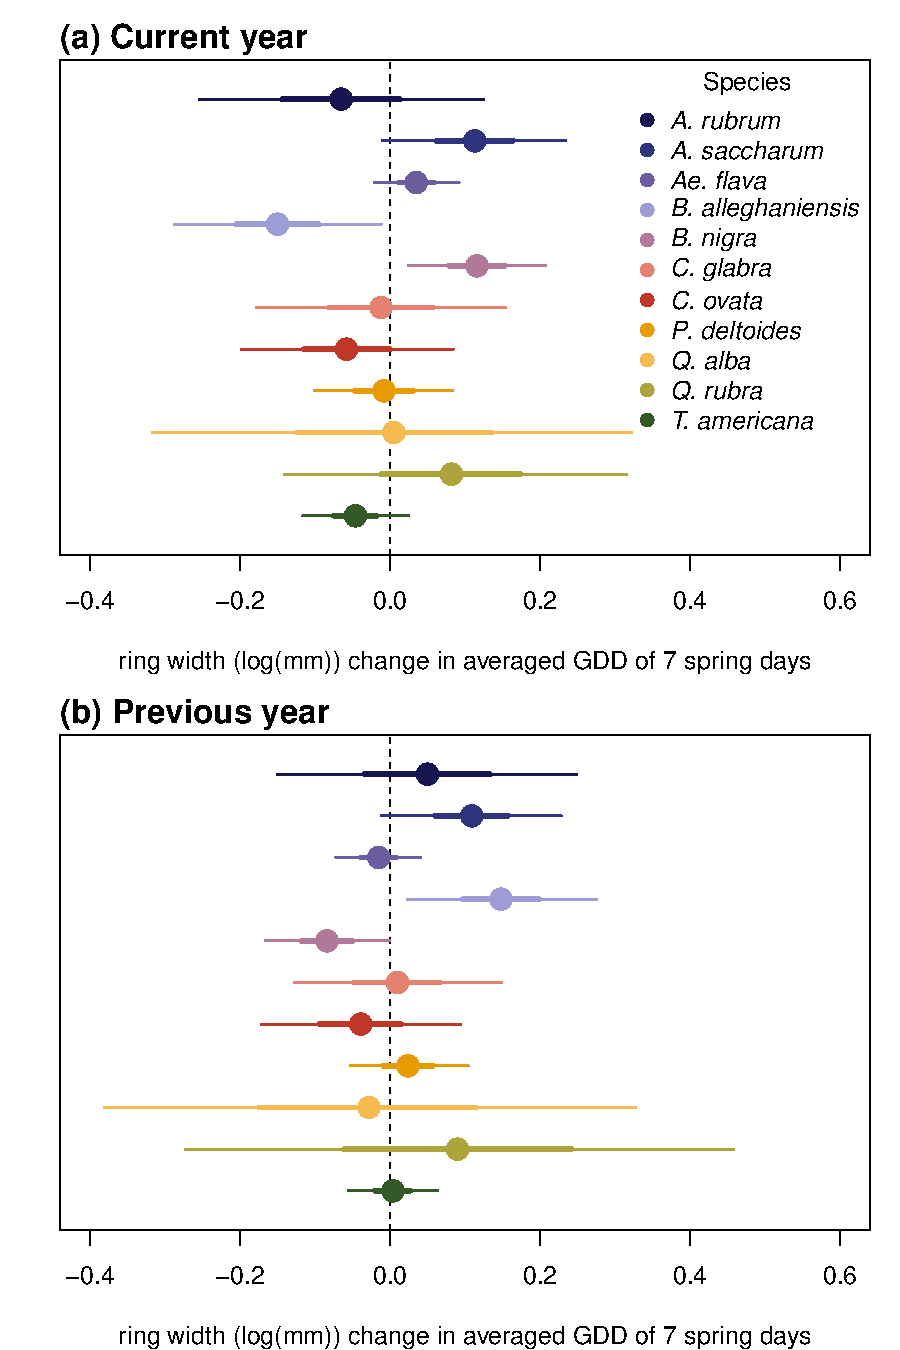
\includegraphics[width=0.6\textwidth]{../../analyses/figures/growthPreviousYearModel/bsppCurrentVSpreviousYR.pdf}
\caption{Model slope estimates representing ring width change as a function of the current year growing degree days (GDD; a) and the previous year GDD (b). GDD represent the accumulated growing degree days between leafout and leaf colouring and the models estimates shows ring width change (on the log scale) per seven average spring days GDD (58.32; see data analyses for more details).
The dots represent the mean of each species and the lines, the 50\% and 90\% uncertainty intervals (UI). }
\label{fig:tsPrvsYr}
\end{figure}

% <><><><><><><><><><><><><><><><><><><><><><><><><><><><><><><><><><><><><><><>
% DISCUSSION
% <><><><><><><><><><><><><><><><><><><><><><><><><><><><><><><><><><><><><><><>
\clearpage
\section*{Discussion}
\begin{enumerate}
% Paragraph
\item Used 49 tress of 11 species to understand if mature trees grew more with longer GS
  \begin{enumerate}
  \item Annual growth with tree rings and leaf phenology for SOS and EOS
  
  \item Warmer and longer GS did not increase growth for any species and decreased growth for one
  
  \item Previous year conditions shifted growth trend for two species
  
  \item Most species did not respond to SOS or EOS
  
  \end{enumerate}

% Paragraph
\item Despite varying growth strategies, no consistent growth trend
  \begin{enumerate}
  \item Thermal or calendar season had no effect on any species except for one
  
  \item {\Ball} decrease in growth reveal that this species growth may be inhibited by warmer seasons
  
  \item {\Ball} response to thermal season is consequential with more growth with earlier EOS: period of high GDD accumulation
  
  \item {\Tame}: grows less with earlier SOS; shows cool early spring days may reduce growth
  
  \item These suggest no difference of current GS condition/length between acquisitive vs conservative species 
  
  \end{enumerate}

% Paragraph
\item Previous year conditions affected growth for two \textit{Betula}
  \begin{enumerate}
  \item Diametrically opposed responses between {\Ball} and {\Bnig}
  
  \item {\Ball} trend suggests that warmer conditions in previous year increases growth, but current decreases
  
  \item Points towards allocation strategy that prioritize storage before growth---expected with conservative species
  
  \item {\Bnig} increases in the current year, but only when previous year is included
  
  \item This highlights the importance of considering not only the current year conditions
  
  \end{enumerate}

% Paragraph
\item Weak responses across species corroborates previous findings on mature deciduous trees
  \begin{enumerate}
  \item Our mature trees don't grow more with warmer or longer seasons 
  
  \item Considering previous year condition is important, which may blur trees responses to current GS length/conditions
  
  \item GS are expected to keep increasing, but tree growth may not follow
  
  \item Temperate forest carbon sink may not keep increasing as expected
  
  \end{enumerate}
  
\end{enumerate}


% <><><><><><><><><><><><><><><><><><><><><><><><><><><><><><><><><><><><><><><>
% Supplemental results
% <><><><><><><><><><><><><><><><><><><><><><><><><><><><><><><><><><><><><><><>
\clearpage
%emw22Jun -- add full model tables ... 
\clearpage
\section*{Supplemental results}

\setcounter{table}{0}
\renewcommand{\thetable}{S\arabic{table}}
\setcounter{figure}{0}
\renewcommand{\thefigure}{S\arabic{figure}}


% latex table generated in R 4.5.1 by xtable 1.8-4 package
% Thu Jul  2 12:49:57 2026
\begin{table}[ht]
\centering
\caption{Species level slope parameters which represent ring width change (on the log scale), per scaled predictor (see data analyses section for more details). We report estimates as mean and 90\% uncertainty intervals (in square brackets) across our four different predictors (GDD: growing degree days, GSL: growing season length, SOS: start of season and EOS: end of season).} 
\label{tab:ts_slope_table}
\begin{tabular}{lllll}
  \hline
Species & GDD & GSL & SOS & EOS \\ 
  \hline
A. rubrum & 0.00 [-0.06, 0.06] & 0.05 [-0.05, 0.15] & -0.05 [-0.28, 0.18] & 0.04 [-0.07, 0.14] \\ 
  A. saccharum & 0.03 [-0.01, 0.07] & 0.00 [-0.04, 0.05] & 0.08 [-0.02, 0.17] & 0.03 [-0.03, 0.08] \\ 
  Ae. flava & 0.01 [-0.01, 0.02] & 0.02 [-0.01, 0.05] & -0.04 [-0.22, 0.13] & 0.02 [-0.01, 0.05] \\ 
  B. alleghaniensis & -0.08 [-0.12, -0.03] & -0.05 [-0.12, 0.02] & -0.08 [-0.23, 0.07] & -0.09 [-0.16, -0.01] \\ 
  B. nigra & 0.03 [-0.00, 0.05] & 0.03 [-0.02, 0.07] & 0.03 [-0.10, 0.16] & 0.03 [-0.02, 0.08] \\ 
  C. glabra & 0.02 [-0.02, 0.06] & 0.03 [-0.03, 0.08] & 0.08 [-0.07, 0.23] & 0.04 [-0.02, 0.09] \\ 
  C. ovata & -0.00 [-0.05, 0.04] & -0.01 [-0.07, 0.05] & 0.10 [-0.03, 0.24] & 0.01 [-0.06, 0.08] \\ 
  P. deltoides & 0.00 [-0.02, 0.03] & 0.02 [-0.03, 0.06] & 0.07 [-0.09, 0.22] & 0.02 [-0.02, 0.06] \\ 
  Q. alba & 0.02 [-0.06, 0.10] & 0.03 [-0.06, 0.13] & 0.00 [-0.18, 0.18] & 0.05 [-0.07, 0.16] \\ 
  Q. rubra & 0.03 [-0.03, 0.09] & 0.03 [-0.08, 0.14] & 0.09 [-0.10, 0.28] & 0.05 [-0.06, 0.15] \\ 
  T. americana & -0.01 [-0.03, 0.01] & -0.02 [-0.05, 0.01] & 0.15 [0.02, 0.27] & -0.01 [-0.04, 0.02] \\ 
   \hline
\end{tabular}
\end{table}



% latex table generated in R 4.5.1 by xtable 1.8-4 package
% Thu Jul  2 12:49:57 2026
\begin{table}[ht]
\centering
\caption{Summary output of each parameter from our four predictors, using ring width (on the log scale) as the reponse variable. We report estimates as mean and 90\% uncertainty intervals (in square brackets) across our four different predictors (GDD: growing degree days, GSL: growing season length, SOS: start of season and EOS: end of season). See data analyses section for more details.} 
\label{tab:tab_all}
\begin{tabular}{lllll}
  \hline
Parameter & GDD & GSL & SOS & EOS \\ 
  \hline
$\alpha$ & 0.61 [-2.08, 3.25] & 0.49 [-2.09, 3.03] & 0.24 [-2.39, 2.94] & 0.23 [-2.48, 2.98] \\ 
  $\sigma_{\alpha_{tree}}$ & 0.55 [0.45, 0.67] & 0.55 [0.45, 0.68] & 0.54 [0.44, 0.66] & 0.55 [0.45, 0.67] \\ 
  $\sigma_{y}$ & 0.31 [0.29, 0.34] & 0.32 [0.29, 0.34] & 0.32 [0.29, 0.34] & 0.32 [0.29, 0.34] \\ 
  $\beta_{spp_{A. rubrum}}$ & 0.00 [-0.06, 0.06] & 0.05 [-0.05, 0.15] & -0.05 [-0.28, 0.18] & 0.04 [-0.07, 0.14] \\ 
  $\beta_{spp_{A. saccharum}}$ & 0.03 [-0.01, 0.07] & 0.00 [-0.04, 0.05] & 0.08 [-0.02, 0.17] & 0.03 [-0.03, 0.08] \\ 
  $\beta_{spp_{Ae. flava}}$ & 0.01 [-0.01, 0.02] & 0.02 [-0.01, 0.05] & -0.04 [-0.22, 0.13] & 0.02 [-0.01, 0.05] \\ 
  $\beta_{spp_{B. alleghaniensis}}$ & -0.08 [-0.12, -0.03] & -0.05 [-0.12, 0.02] & -0.08 [-0.23, 0.07] & -0.09 [-0.16, -0.01] \\ 
  $\beta_{spp_{B. nigra}}$ & 0.03 [-0.00, 0.05] & 0.03 [-0.02, 0.07] & 0.03 [-0.10, 0.16] & 0.03 [-0.02, 0.08] \\ 
  $\beta_{spp_{C. glabra}}$ & 0.02 [-0.02, 0.06] & 0.03 [-0.03, 0.08] & 0.08 [-0.07, 0.23] & 0.04 [-0.02, 0.09] \\ 
  $\beta_{spp_{C. ovata}}$ & -0.00 [-0.05, 0.04] & -0.01 [-0.07, 0.05] & 0.10 [-0.03, 0.24] & 0.01 [-0.06, 0.08] \\ 
  $\beta_{spp_{P. deltoides}}$ & 0.00 [-0.02, 0.03] & 0.02 [-0.03, 0.06] & 0.07 [-0.09, 0.22] & 0.02 [-0.02, 0.06] \\ 
  $\beta_{spp_{Q. alba}}$ & 0.02 [-0.06, 0.10] & 0.03 [-0.06, 0.13] & 0.00 [-0.18, 0.18] & 0.05 [-0.07, 0.16] \\ 
  $\beta_{spp_{Q. rubra}}$ & 0.03 [-0.03, 0.09] & 0.03 [-0.08, 0.14] & 0.09 [-0.10, 0.28] & 0.05 [-0.06, 0.15] \\ 
  $\beta_{spp_{T. americana}}$ & -0.01 [-0.03, 0.01] & -0.02 [-0.05, 0.01] & 0.15 [0.02, 0.27] & -0.01 [-0.04, 0.02] \\ 
  $\alpha_{year_{2019}}$ & 0.09 [-0.46, 0.64] & 0.06 [-0.48, 0.63] & 0.07 [-0.47, 0.64] & 0.06 [-0.50, 0.62] \\ 
  $\alpha_{year_{2020}}$ & -0.06 [-0.60, 0.49] & -0.07 [-0.61, 0.50] & -0.12 [-0.66, 0.45] & -0.07 [-0.63, 0.47] \\ 
  $\alpha_{year_{2021}}$ & 0.00 [-0.55, 0.56] & -0.00 [-0.55, 0.57] & 0.01 [-0.54, 0.58] & -0.01 [-0.58, 0.54] \\ 
  $\alpha_{year_{2022}}$ & -0.05 [-0.61, 0.50] & -0.07 [-0.63, 0.50] & -0.07 [-0.63, 0.49] & -0.08 [-0.65, 0.48] \\ 
  $\alpha_{year_{2023}}$ & 0.20 [-0.36, 0.76] & 0.18 [-0.38, 0.75] & 0.20 [-0.35, 0.78] & 0.17 [-0.40, 0.72] \\ 
  $\alpha_{year_{2024}}$ & 0.08 [-0.47, 0.64] & 0.07 [-0.47, 0.66] & 0.07 [-0.48, 0.64] & 0.08 [-0.49, 0.64] \\ 
  $\alpha_{year_{2016}}$ & -0.21 [-0.77, 0.34] & -0.22 [-0.76, 0.35] & -0.25 [-0.80, 0.31] & -0.25 [-0.81, 0.29] \\ 
  $\alpha_{year_{2017}}$ & -0.03 [-0.58, 0.52] & -0.06 [-0.59, 0.52] & 0.00 [-0.54, 0.56] & -0.07 [-0.63, 0.48] \\ 
  $\alpha_{year_{2018}}$ & 0.04 [-0.52, 0.59] & 0.02 [-0.52, 0.59] & -0.00 [-0.55, 0.56] & 0.01 [-0.54, 0.56] \\ 
  $\alpha_{spp_{A. rubrum}}$ & -0.05 [-3.40, 3.35] & -0.95 [-4.12, 2.17] & 1.23 [-3.23, 5.60] & -1.08 [-5.62, 3.44] \\ 
  $\alpha_{spp_{A. saccharum}}$ & -0.90 [-3.86, 2.10] & 0.43 [-2.34, 3.17] & -0.57 [-3.59, 2.35] & -0.37 [-3.79, 3.02] \\ 
  $\alpha_{spp_{Ae. flava}}$ & -0.49 [-3.20, 2.19] & -0.46 [-3.09, 2.14] & 0.93 [-2.69, 4.47] & -0.49 [-3.33, 2.38] \\ 
  $\alpha_{spp_{B. alleghaniensis}}$ & 2.32 [-0.68, 5.34] & 0.61 [-2.29, 3.46] & 1.17 [-2.34, 4.58] & 3.25 [-0.47, 6.96] \\ 
  $\alpha_{spp_{B. nigra}}$ & -0.68 [-3.54, 2.12] & -0.13 [-2.82, 2.58] & 0.17 [-3.18, 3.40] & -0.50 [-3.65, 2.67] \\ 
  $\alpha_{spp_{C. glabra}}$ & -0.89 [-3.89, 2.06] & -0.64 [-3.44, 2.12] & -1.17 [-4.65, 2.33] & -1.16 [-4.46, 2.12] \\ 
  $\alpha_{spp_{C. ovata}}$ & -0.32 [-3.35, 2.74] & -0.07 [-2.88, 2.73] & -1.96 [-5.42, 1.40] & -0.35 [-4.01, 3.29] \\ 
  $\alpha_{spp_{P. deltoides}}$ & -0.38 [-3.14, 2.40] & -0.39 [-3.09, 2.26] & -1.04 [-4.60, 2.52] & -0.49 [-3.54, 2.50] \\ 
  $\alpha_{spp_{Q. alba}}$ & -0.85 [-4.70, 3.03] & -0.56 [-3.66, 2.52] & 0.40 [-3.47, 4.32] & -1.44 [-6.32, 3.48] \\ 
  $\alpha_{spp_{Q. rubra}}$ & -1.09 [-4.47, 2.23] & -0.43 [-3.80, 2.96] & -1.08 [-4.98, 2.91] & -1.44 [-6.04, 3.22] \\ 
  $\alpha_{spp_{T. americana}}$ & 0.30 [-2.41, 3.02] & 0.59 [-1.98, 3.18] & -2.02 [-5.24, 1.14] & 0.92 [-1.93, 3.81] \\ 
   \hline
\end{tabular}
\end{table}


% Coringtreespotters year mu plot
\begin{figure}[!ht]
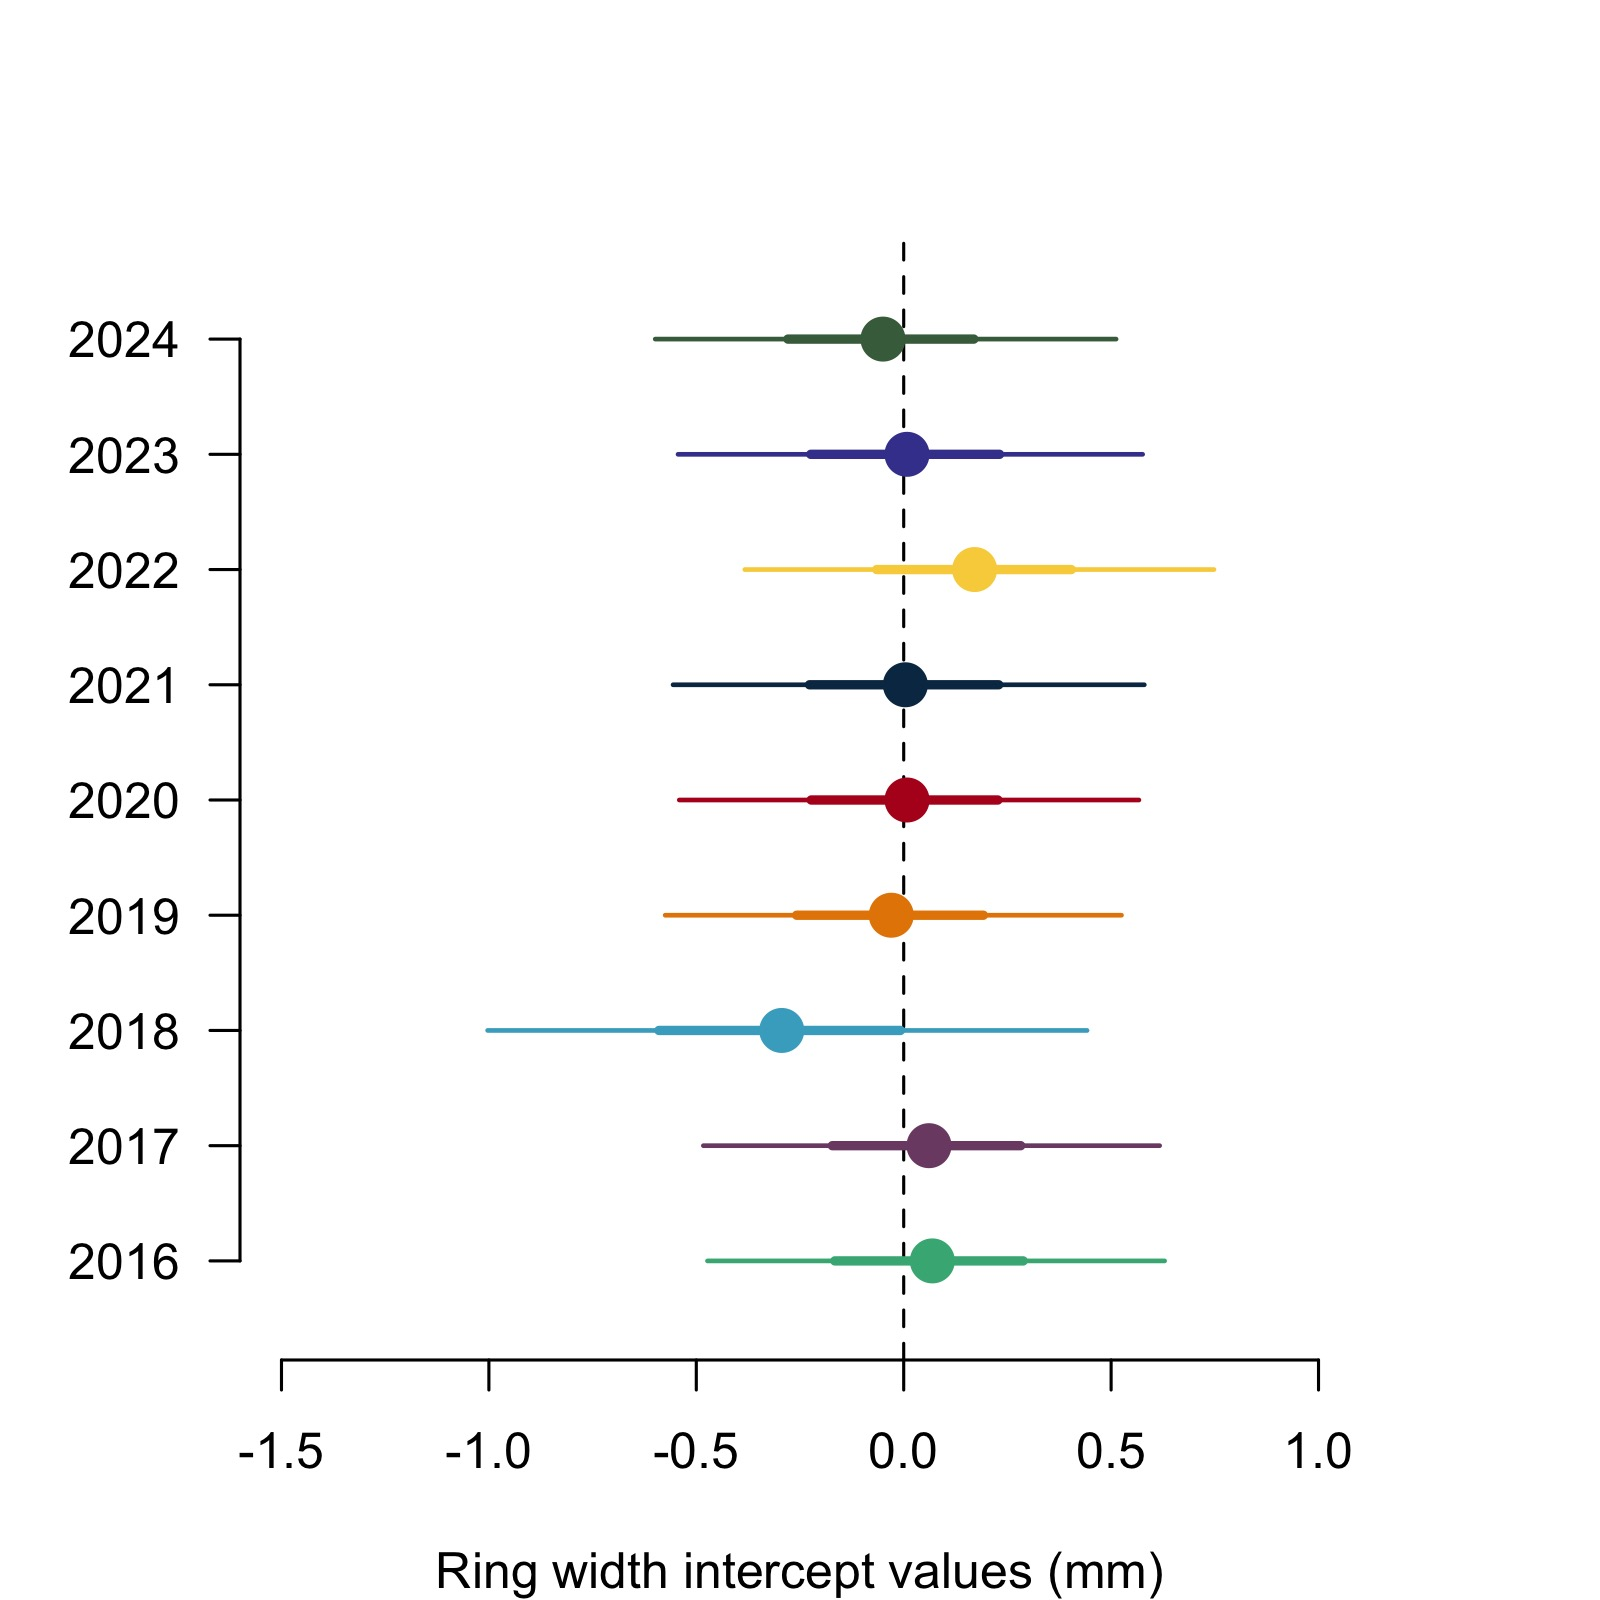
\includegraphics[width=0.5\textwidth]{../../analyses/figures/growthModelsMain/TSmuayear.jpeg}
\caption{Ring width (on the log scale) deviations from the grand mean for each year using the GDD model (Table \ref{tab:tab_all}). The dots are the mean of the posterior distribution and the thick and thin lines, the 50 and 90\% UI.}
\label{fig:tsmuplotayear}
\end{figure}

% Coringtreespotters boxplot
\begin{figure}[!ht]
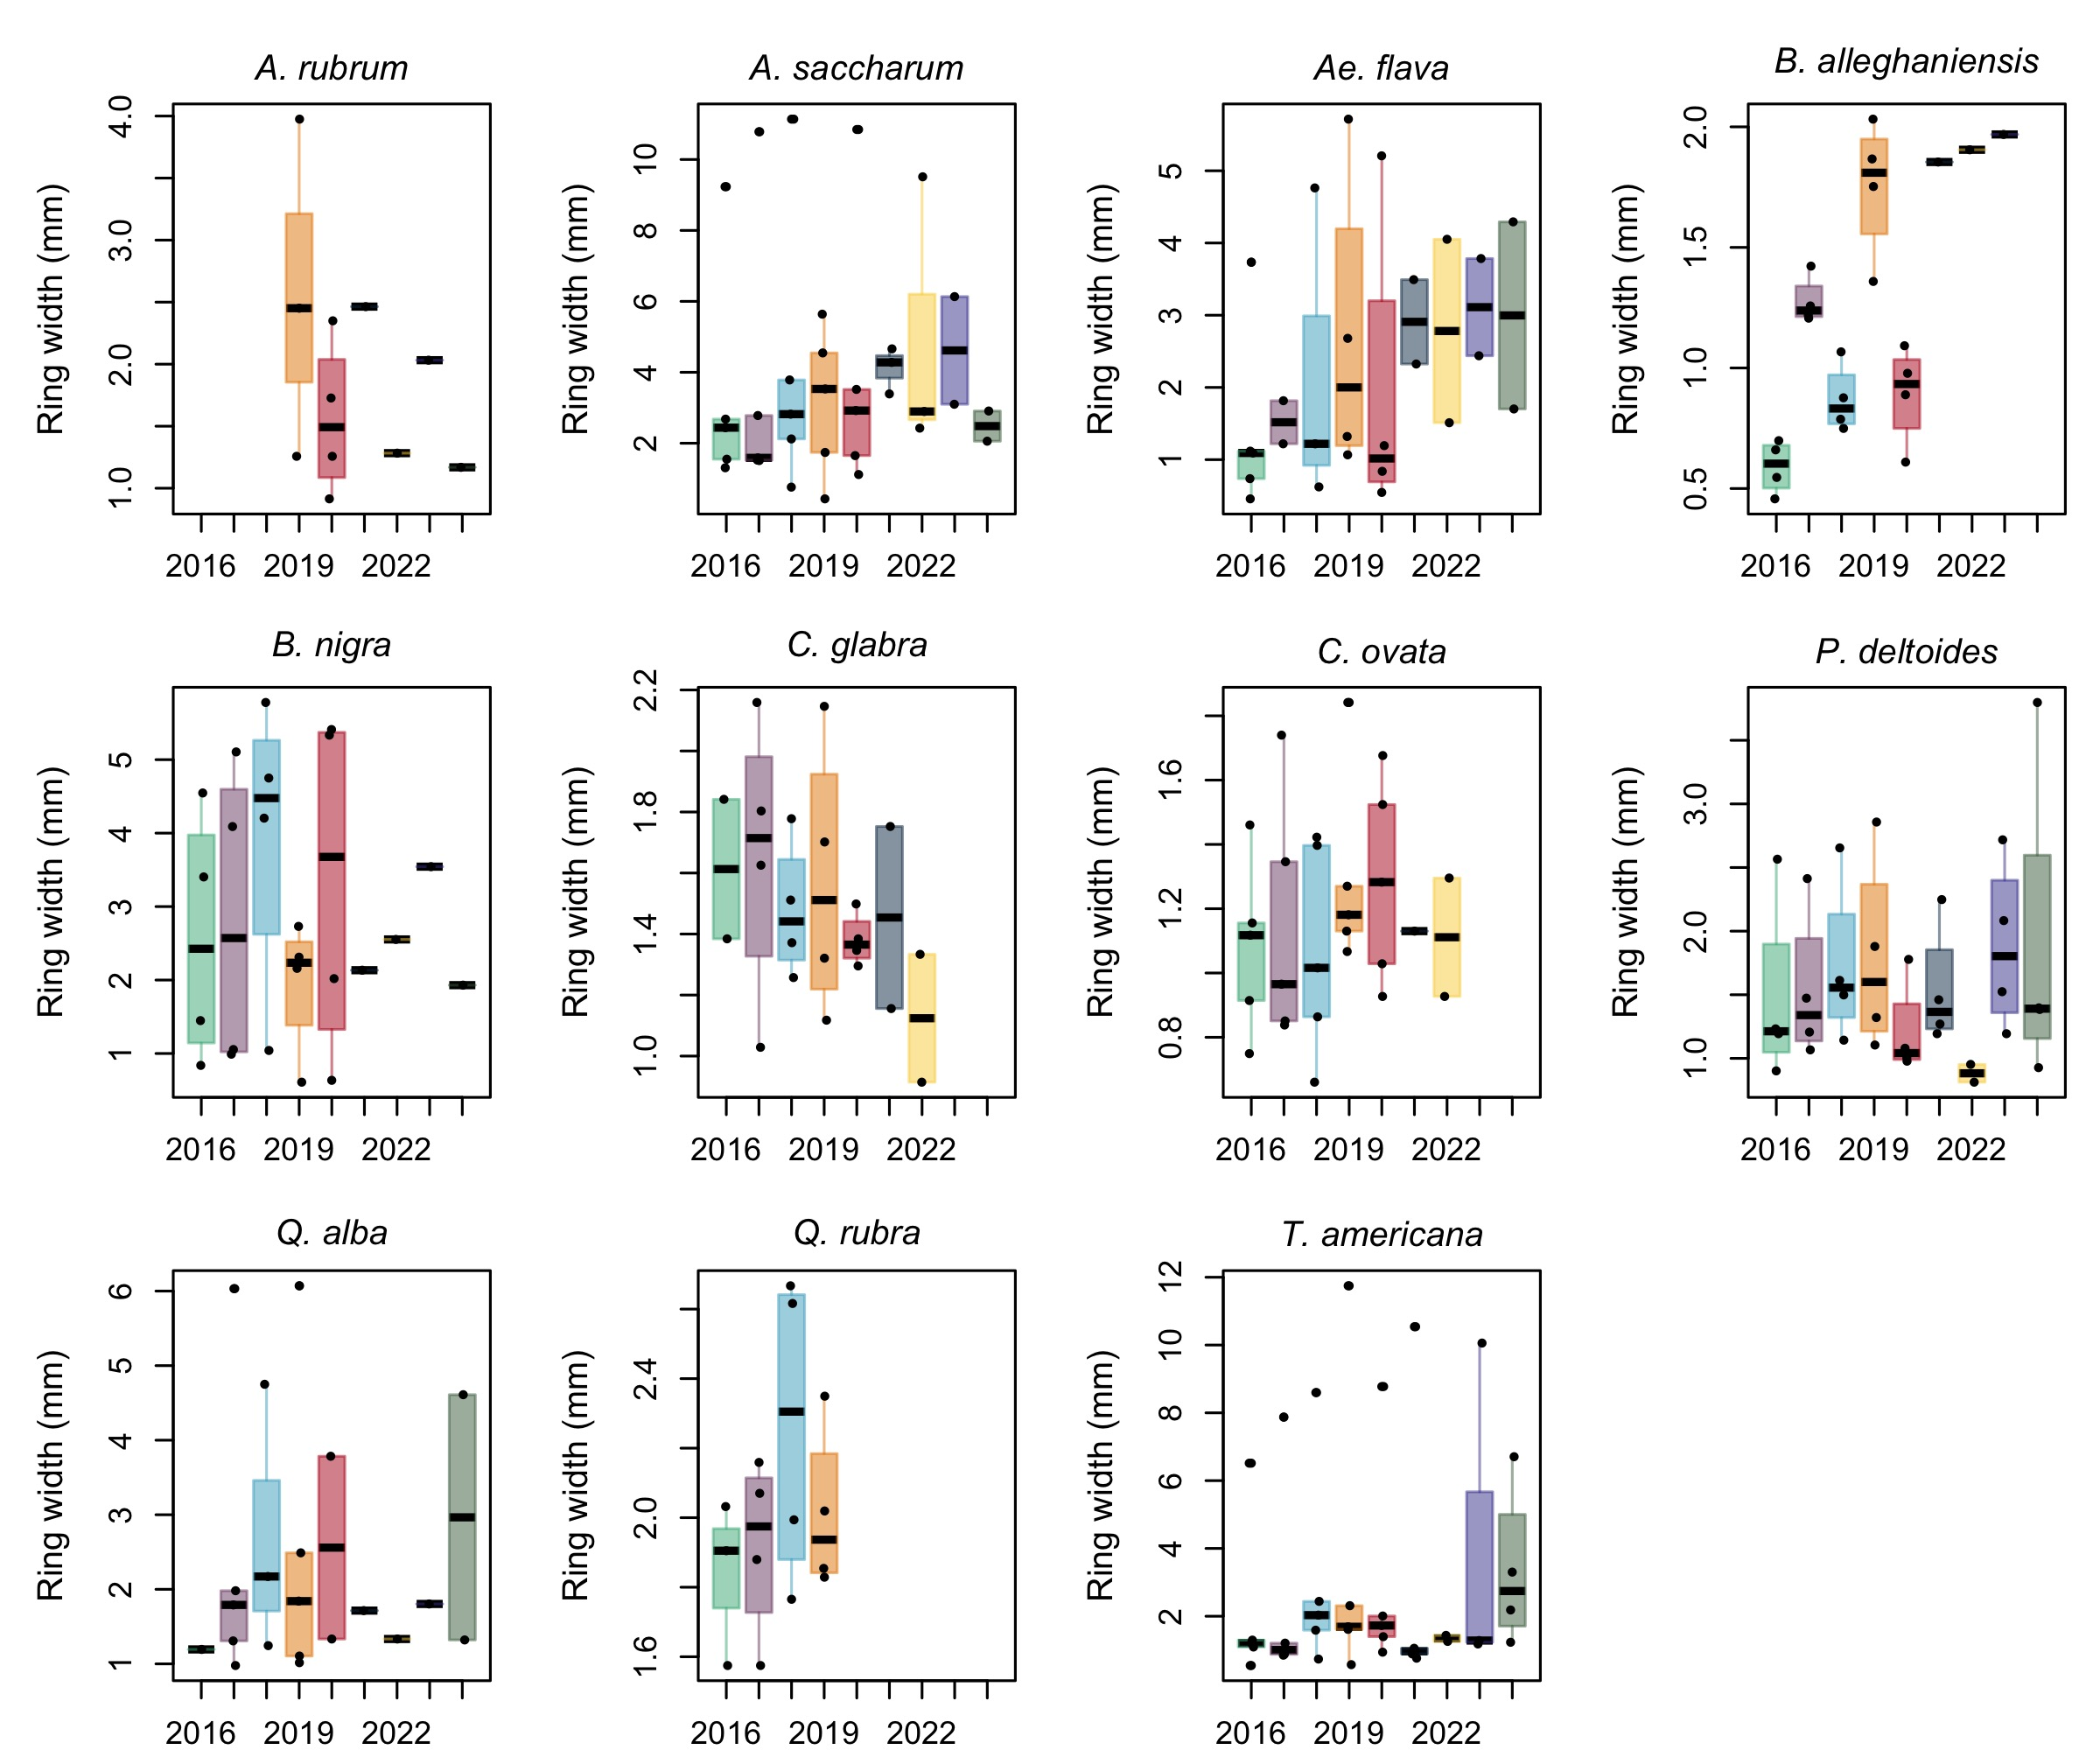
\includegraphics[width=1\textwidth]{../../analyses/figures/growthModelsMain/boxplotRingWidth.jpeg}
\caption{Boxplot representing the empirical data of our ring widths (mm) across years, facetted by species. The dots represent the raw data, the line the mean and the box the interquantile range (IQR).}
\label{fig:tsboxplot}
\end{figure}

% XY facetted by species GDD shaped by tree id
\begin{figure}[!ht]
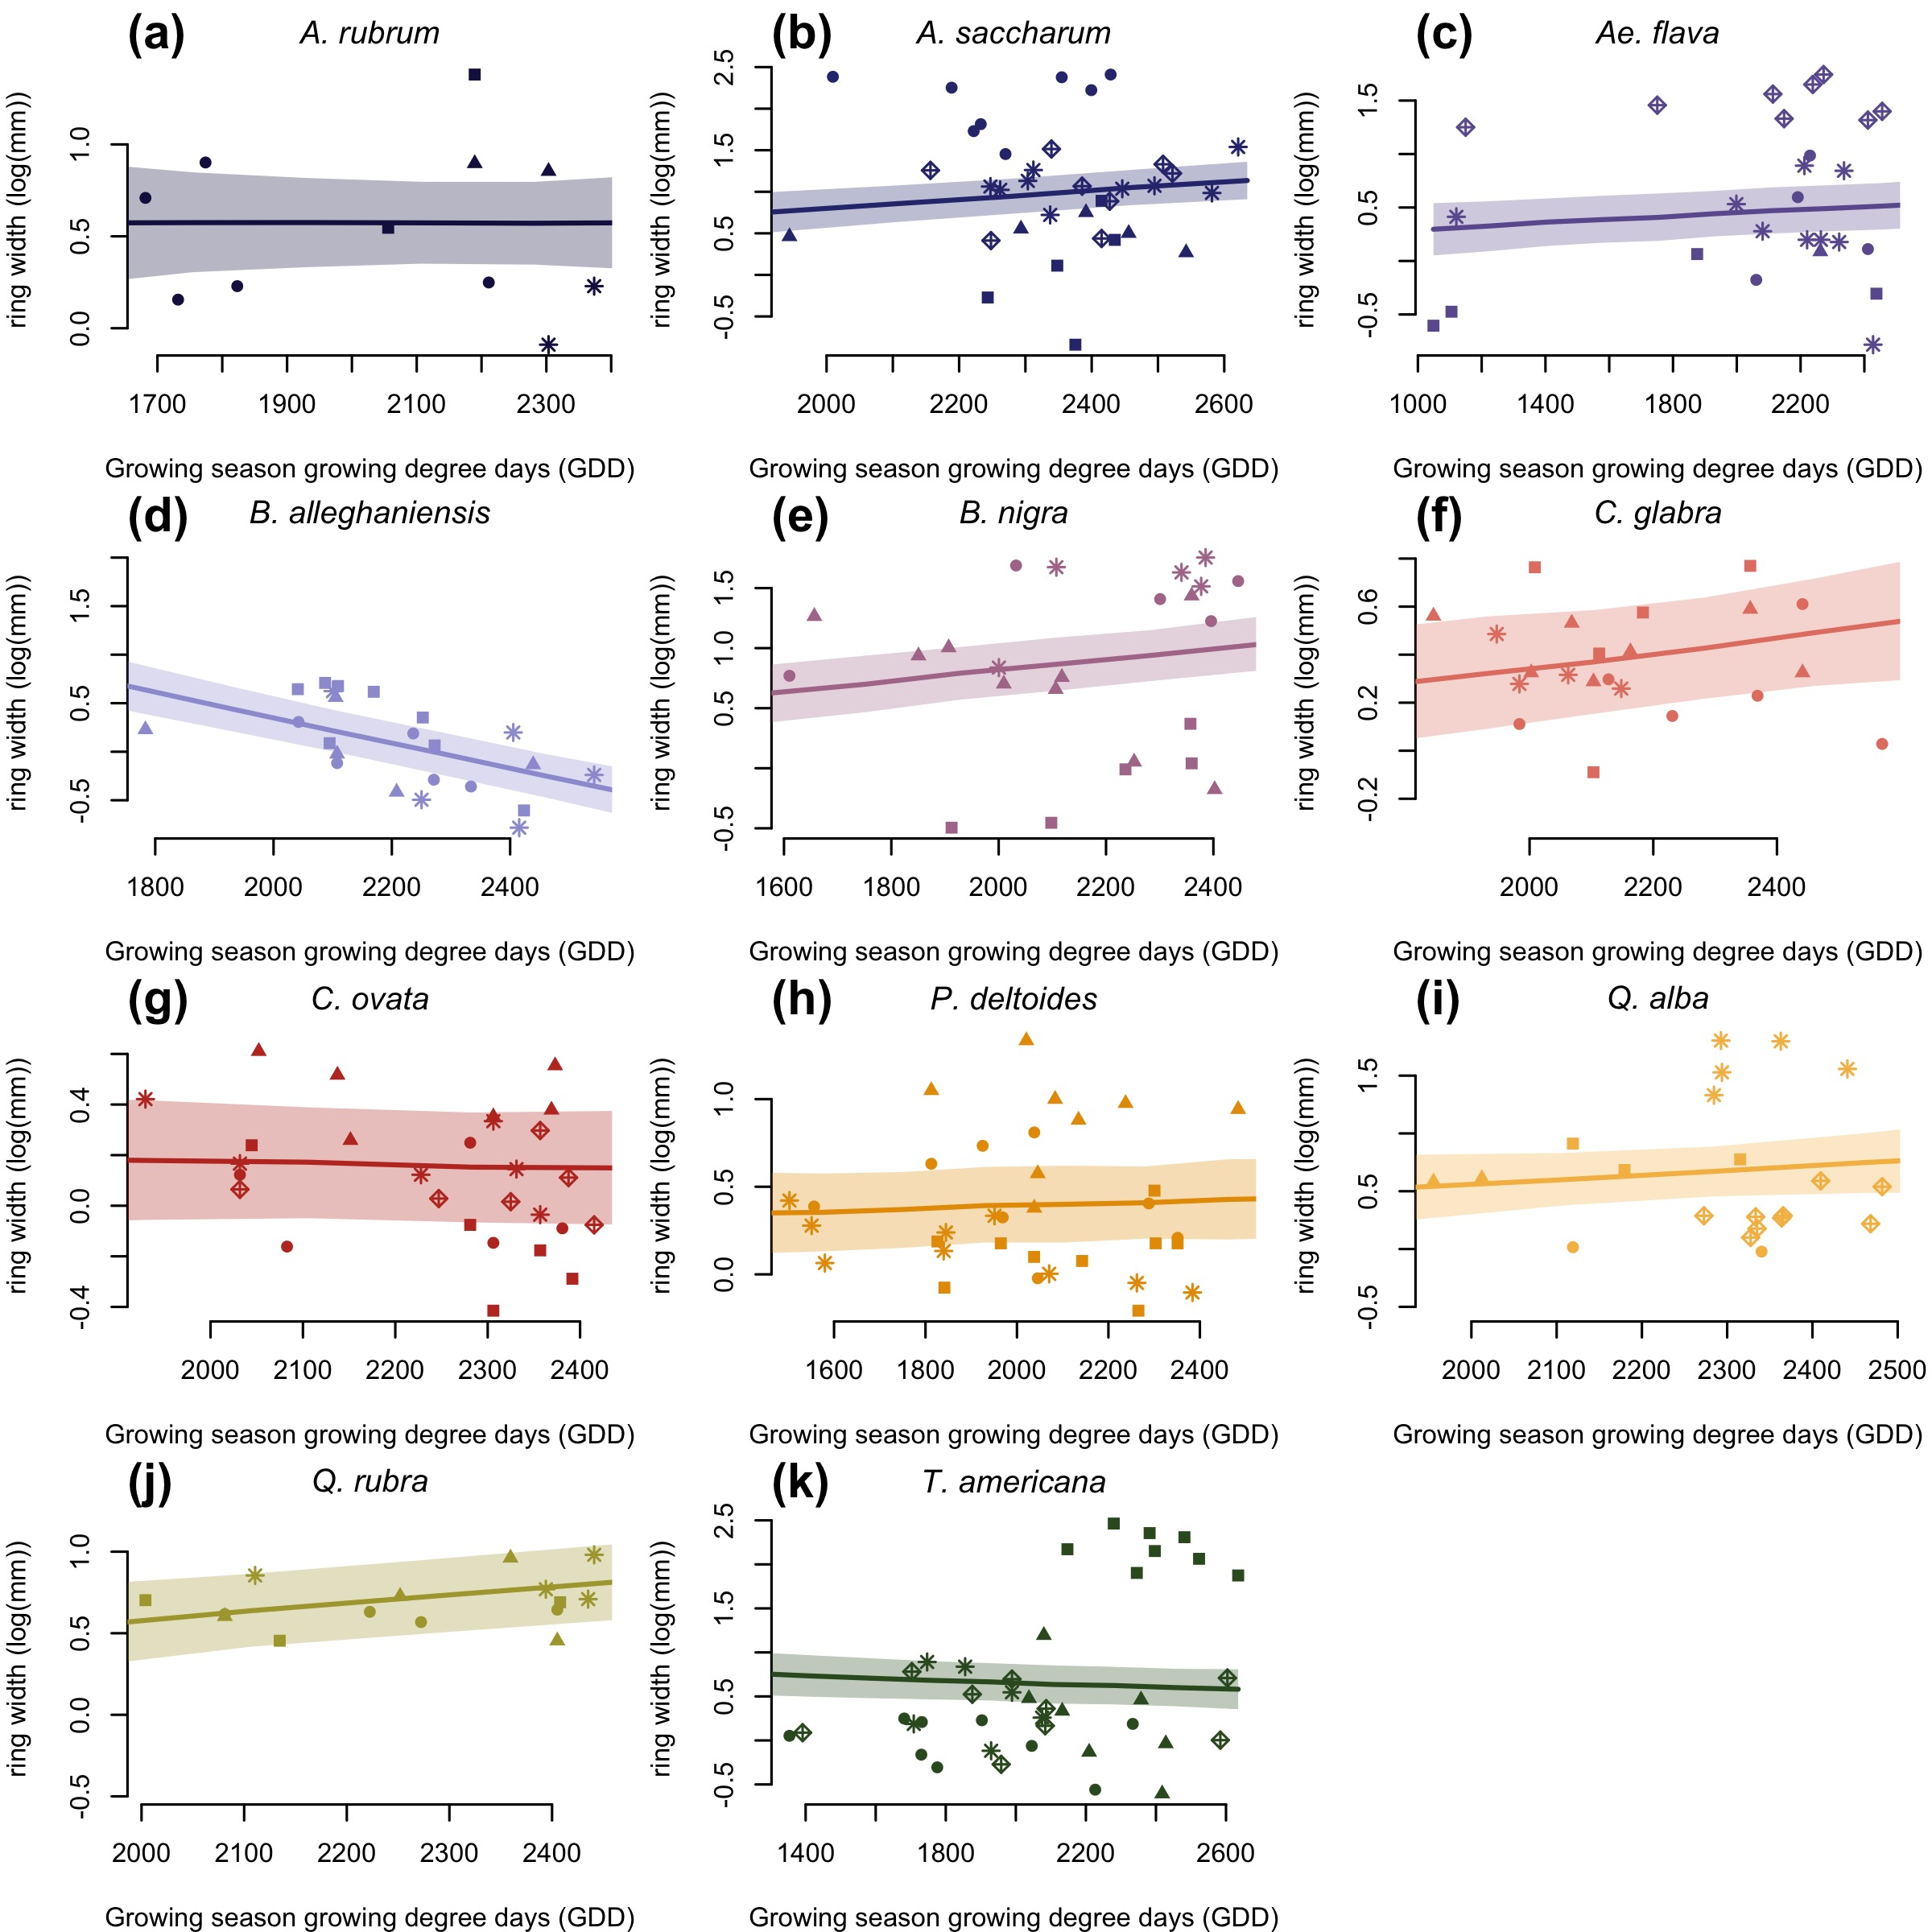
\includegraphics[width=0.8\textwidth]{../../analyses/figures/growthModelsMain/TSgrowthModelSlopesperSppFacetGDDtree.jpeg}
\caption{Ring width (on the log scale) trends in response to thermal season (GDD). The plots are the reconstructed species estimates posterior distribution with error. The lines represent the mean of the posterior distribution and the shaded area, the 50\% UI. The dots are the empirical data shaped by treeids.}
\label{fig:tsxyGDDtree}
\end{figure}

% XY facetted by species GSL shaped by tree id
\begin{figure}[!ht]
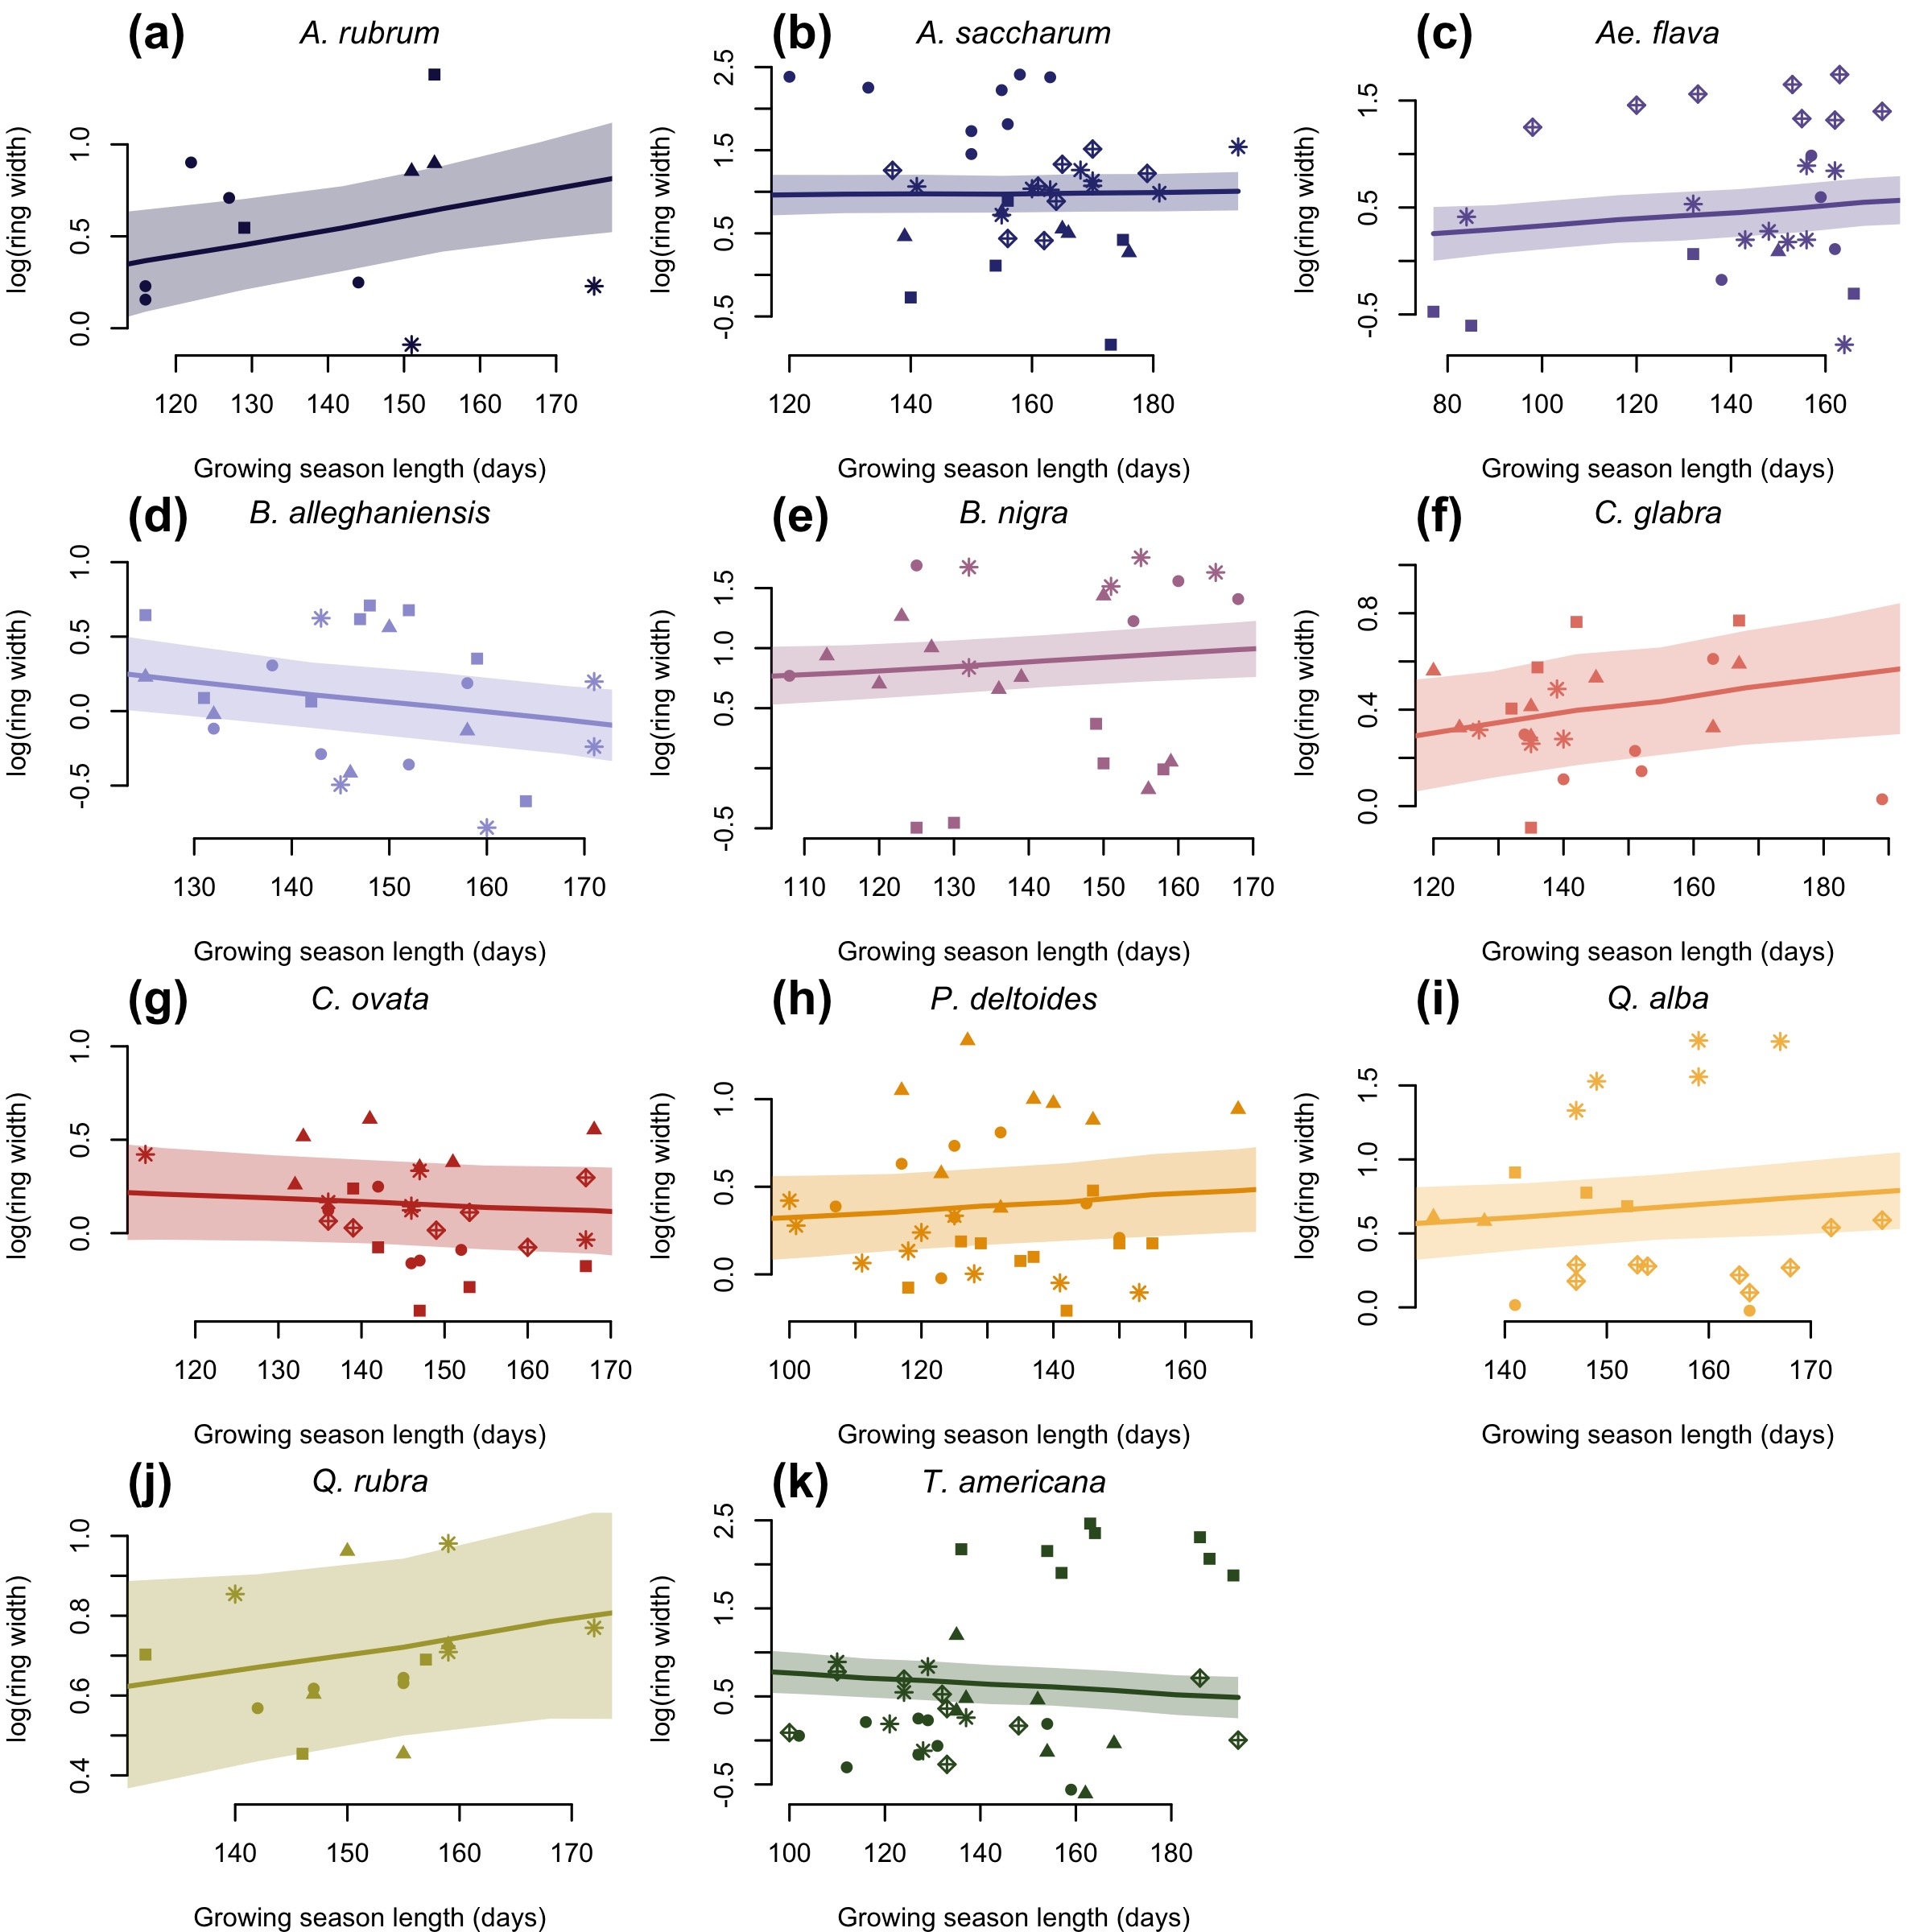
\includegraphics[width=0.8\textwidth]{../../analyses/figures/growthModelsMain/TSgrowthModelSlopesperSppFacetGSLtree.jpeg}
\caption{Ring width trends (on the log scale) in response to calendar season (GSL). The plots are the reconstructed species estimates posterior distribution with error. The lines represent the mean of the posterior distribution and the shaded area, the 50\% UI. The dots are the empirical data shaped by treeids.}
\label{fig:tsxyGSLtree}
\end{figure}

% XY facetted by species GDD shaped by year
\begin{figure}[!ht]
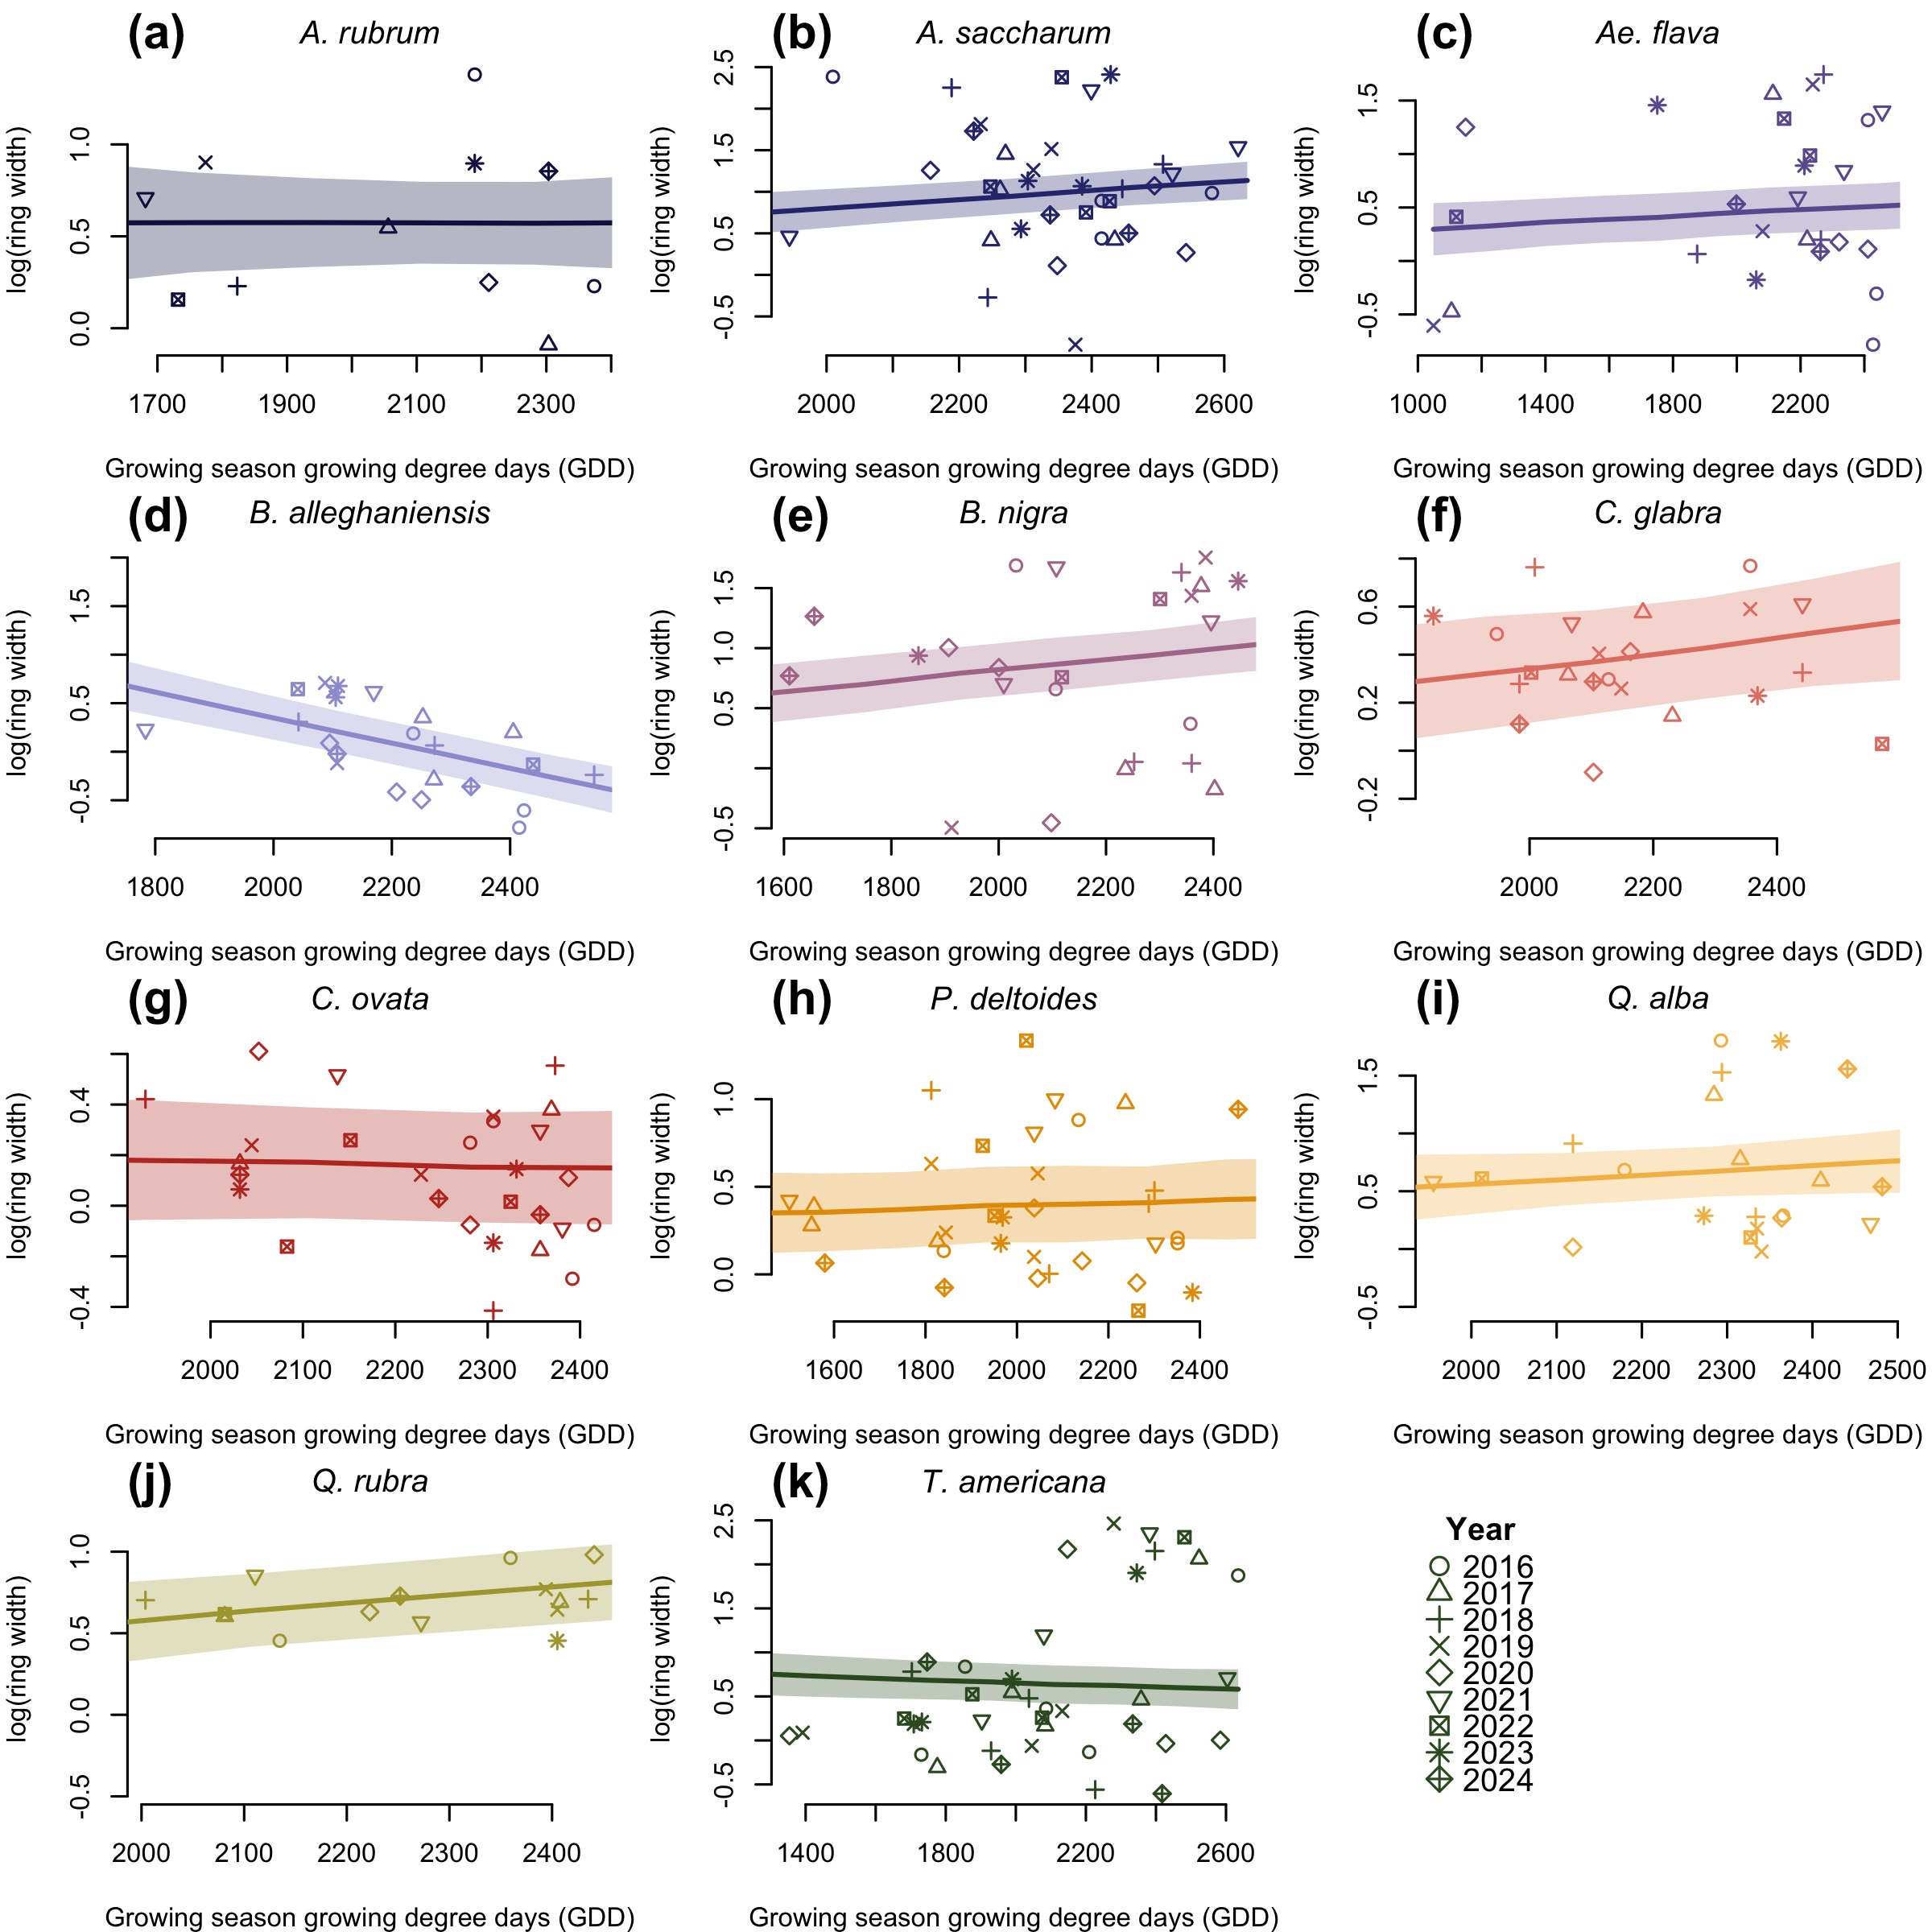
\includegraphics[width=0.8\textwidth]{../../analyses/figures/growthModelsMain/TSgrowthModelSlopesperSppFacetGDDyr.jpeg}
\caption{Ring width trends (on the log scale) in response to thermal season (GDD). The plots are the reconstructed species estimates posterior distribution with error. The lines represent the mean of the posterior distribution and the shaded area, the 50\% UI. The dots are the empirical data shaped by year.}
\label{fig:tsxyGDDyr}
\end{figure}

% XY facetted by species GSL shaped by year
\begin{figure}[!ht]
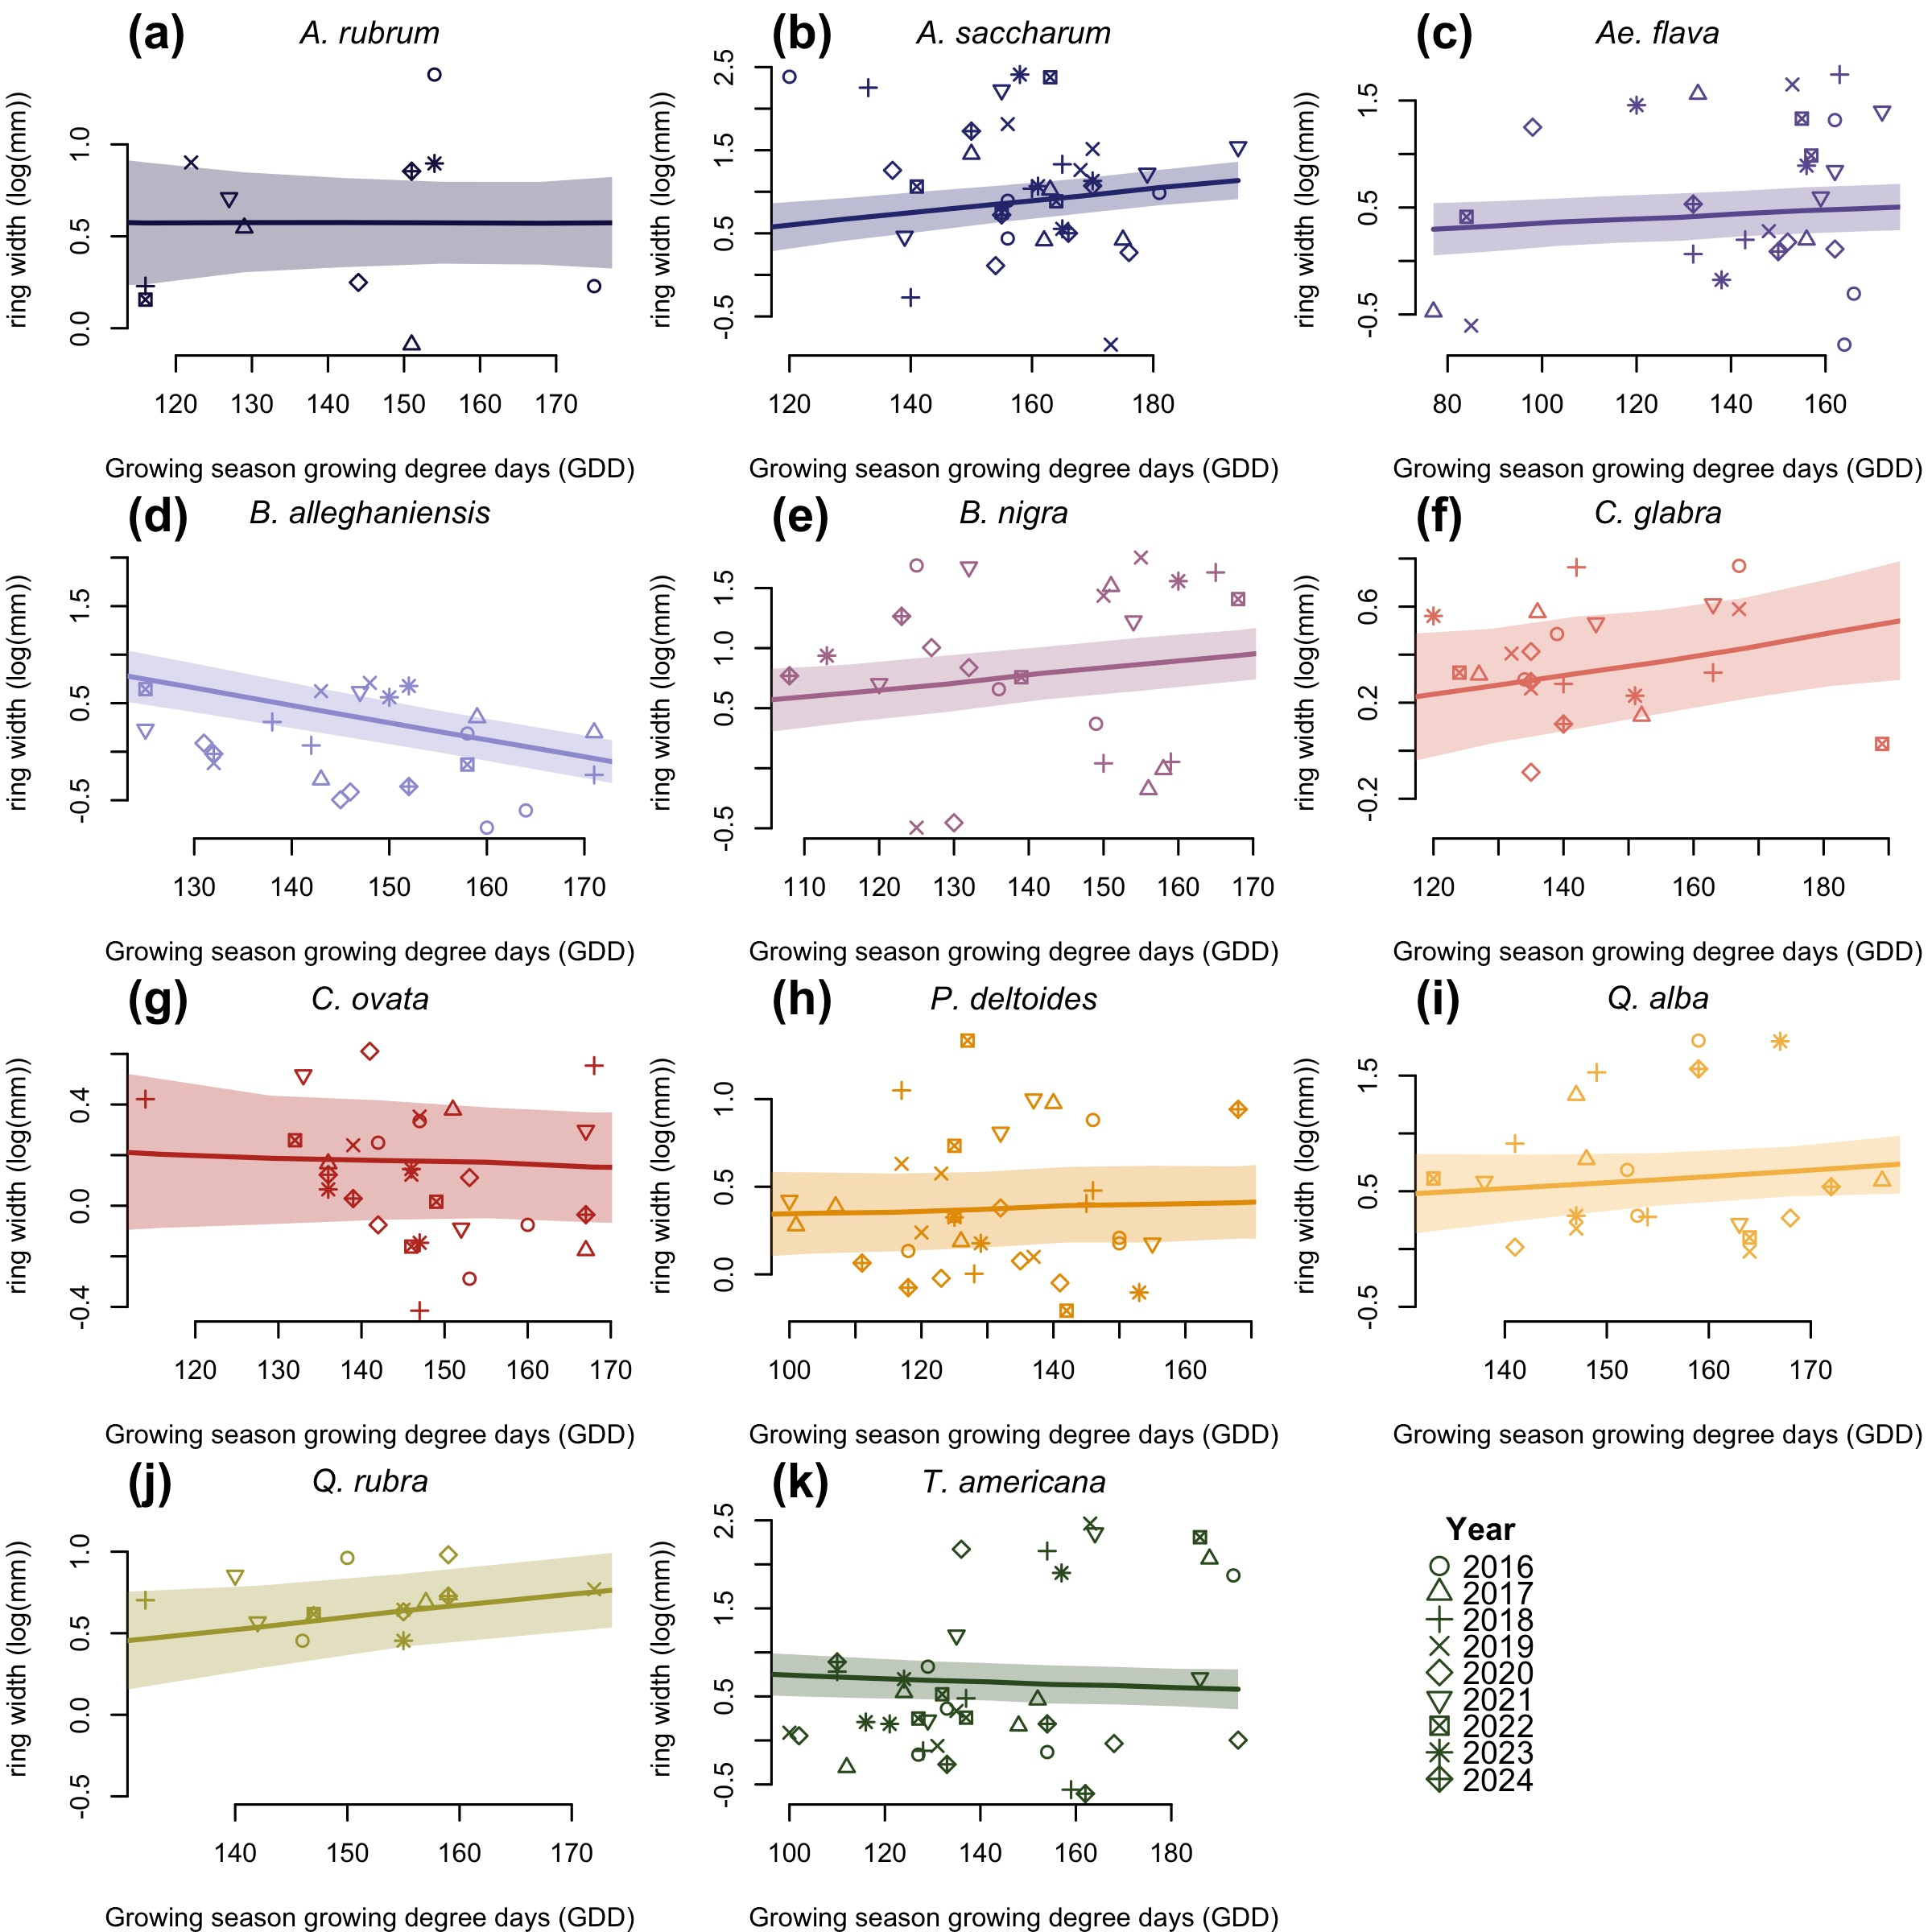
\includegraphics[width=0.8\textwidth]{../../analyses/figures/growthModelsMain/TSgrowthModelSlopesperSppFacetGSLyr.jpeg}
\caption{Ring width trends (on the log scale) in response to calendar season (GSL). The plots are the reconstructed species estimates posterior distribution with error. The lines represent the mean of the posterior distribution and the shaded area, the 50\% UI. The dots are the empirical data shaped by year.}
\label{fig:tsxyGSLyr}
\end{figure}

% Figure mu atreeid full
\begin{figure}[!ht]
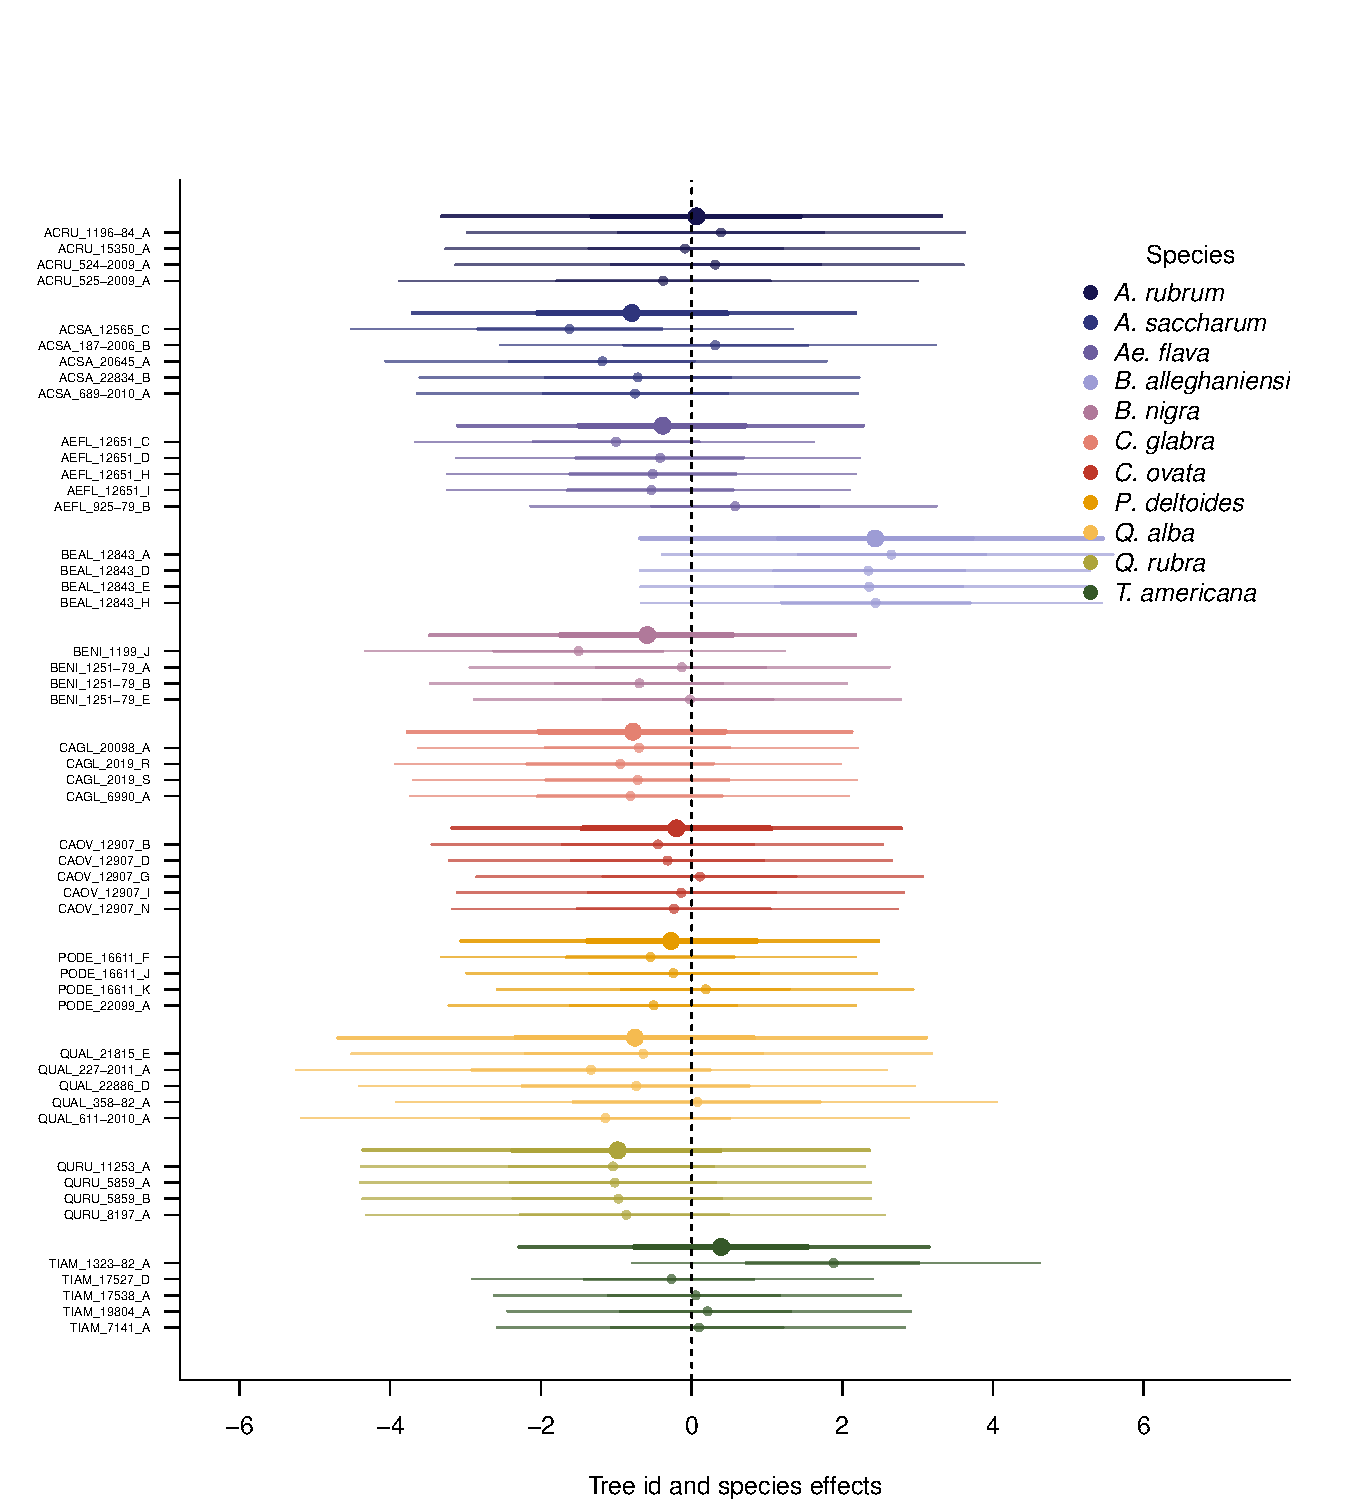
\includegraphics[width=0.8\textwidth]{../../analyses/figures/growthModelsMain/TSmeanPlotGrowthGDD_treeidBYspp.pdf}
\caption{Ring width (on the log scale) deviations from the grand mean for each grouping factor of the GDD model. The different tree id values represent the combined intercepts of tree id, species and averaged year intercepts. The larger dots and lines represent the species intercepts which are the species level estimates averaged across all of their tree ids. The dots are the mean of the posterior distribution and the thick and thin lines, the 50 and 90\% UI.}
\label{fig:tsmuplotatreeid}
\end{figure}

% Full vs restricted data comparison for Coringtreespotters
\begin{figure}[!ht]

\includegraphics[width=1\textwidth]{/Users/christophe_rouleau-desrochers/github/coringtreespotters/analyses/figures/growthModelsMain/FullVSRestricted.pdf}
\caption{Full vs most restricted rows of data for the model with SOS (a) EOS (b) as the predictor. Each pannel represent the different parameters used to fit the models (see data analyses for more details).}
\label{fig:tsSOSEOScomparison}
\end{figure}

% Budburst vs leafout for CoringTreespotters
\begin{figure}[!ht]

\includegraphics[width=0.8\textwidth]{/Users/christophe_rouleau-desrochers/github/coringtreespotters/analyses/figures/growthModelsMain/budburstVSLeafout/DporousVSRporous.jpeg}
\caption{Parameter estimates when calculating the GDD (a), GSL (b) from leafout vs budburst, to leaf coloring. (c) shows the model estimates when taking leafout vs budburst as the SOS (see data analyses for more details).}
\label{fig:buburstVSleafoutTS}
\end{figure}

% Z-scored slope results
\begin{figure}[!ht]
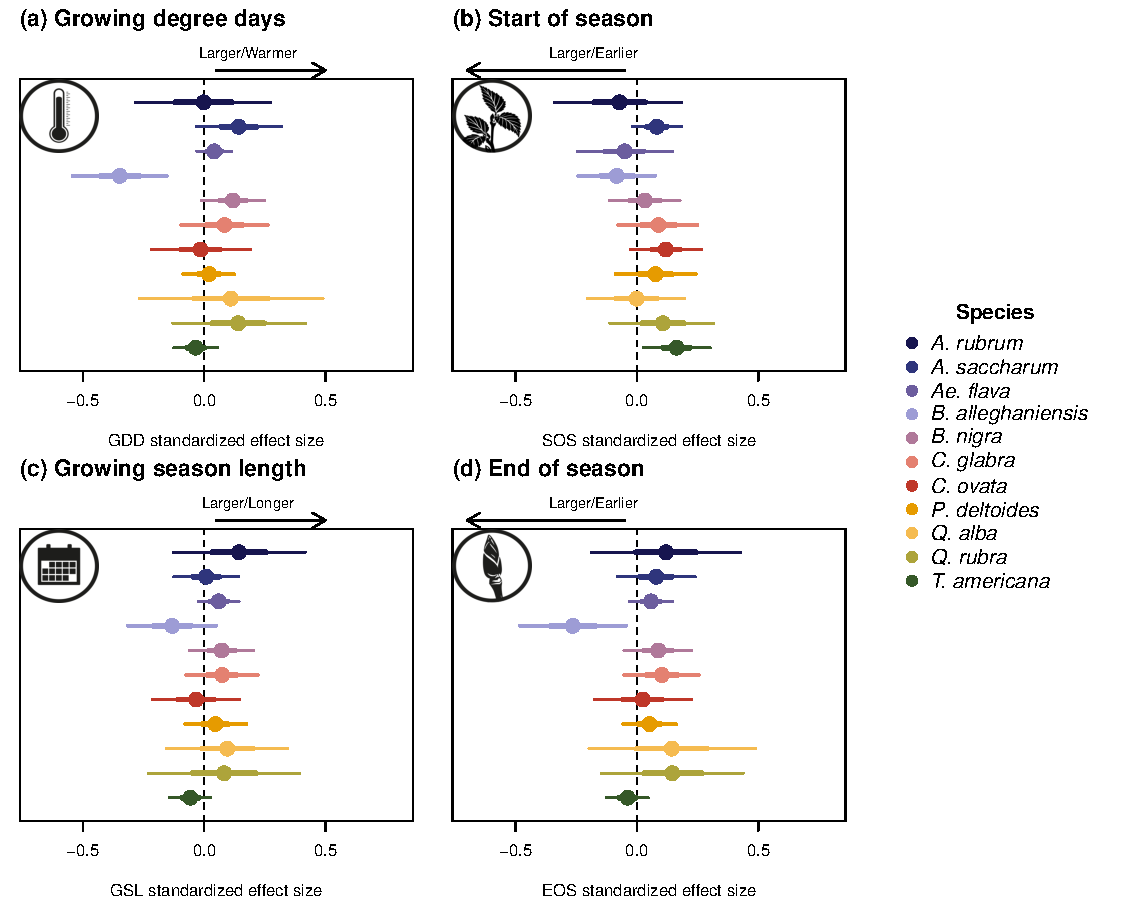
\includegraphics[width=0.8\textwidth]{../../analyses/figures/growthModelsMain/zscored/muALLbsppZ.pdf}
\caption{Effect size of each predictors across our eleven species. We depict ring width (on the log scale) change per scaled (z-scored; see data analyses section for more details) predictor for each species. We report estimates as mean and 90\% uncertainty intervals (in square brackets) across our four different predictors (GDD: growing degree days, GSL: growing season length, SOS: start of season and EOS: end of season).}
\label{fig:bsppZscored}
\end{figure}

% Carry over of SOS on EOS
\begin{figure}[!ht]
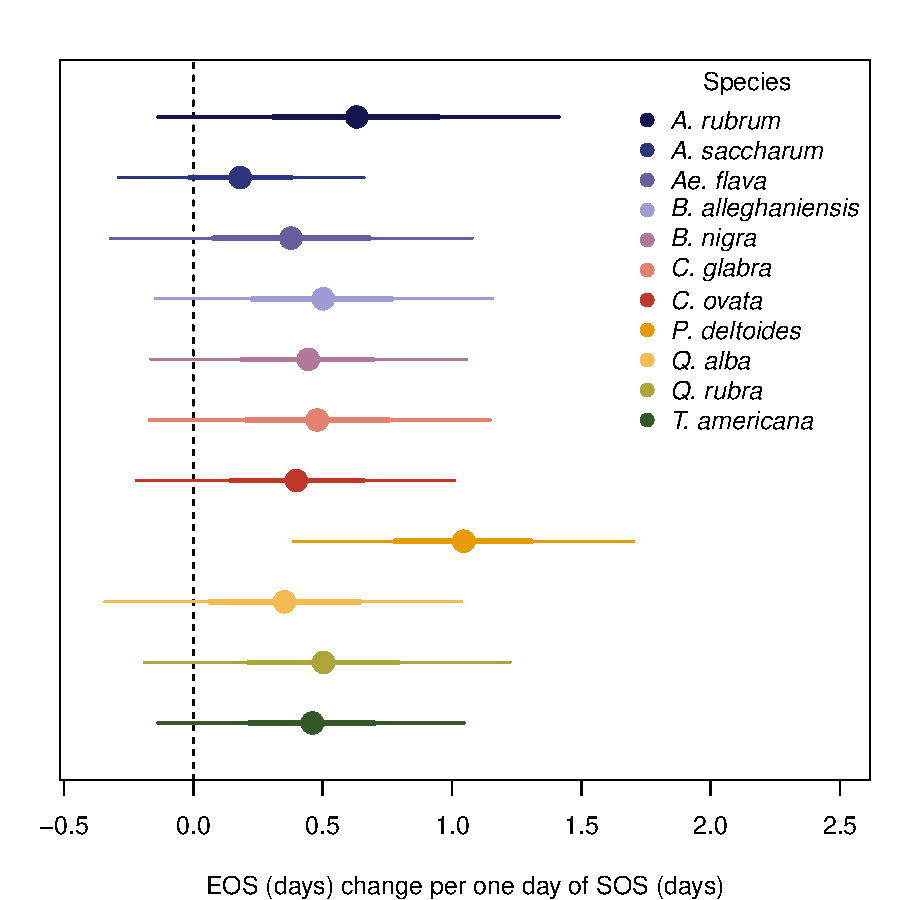
\includegraphics[width=0.8\textwidth]{../../analyses/figures/SOSonEOS/bsppSOSonEOS.pdf}
\caption{Effect of the start of season (SOS) on the end of season (EOS) across our eleven species. We report these slope estimates as mean and 90\% uncertainty intervals.}
\label{fig:SOSonEOS}
\end{figure}

%<><><><><><><><><><><><><><><><><><><><><><><><><><><><><><><><><><><><><><><><>
% REFERENCES %
%<><><><><><><><><><><><><><><><><><><><><><><><><><><><><><><><><><><><><><><><>
\clearpage
\bibliography{ExportedItems}
\bibliographystyle{besjournals} 

\end{document}
